%% Based on a TeXnicCenter-Template by Tino Weinkauf.
%%%%%%%%%%%%%%%%%%%%%%%%%%%%%%%%%%%%%%%%%%%%%%%%%%%%%%%%%%%%%

%%%%%%%%%%%%%%%%%%%%%%%%%%%%%%%%%%%%%%%%%%%%%%%%%%%%%%%%%%%%%
%% HEADER
%%%%%%%%%%%%%%%%%%%%%%%%%%%%%%%%%%%%%%%%%%%%%%%%%%%%%%%%%%%%%
\documentclass[letterpaper,oneside,12pt]{report}
% Alternative Options:
%	Paper Size: a4paper / a5paper / b5paper / letterpaper / legalpaper / executivepaper
% Duplex: oneside / twoside
% Base Font Size: 10pt / 11pt / 12pt


%% Language %%%%%%%%%%%%%%%%%%%%%%%%%%%%%%%%%%%%%%%%%%%%%%%%%
\usepackage[USenglish]{babel} %francais, polish, spanish, ...
\usepackage[T1]{fontenc}
\usepackage[ansinew]{inputenc}

\usepackage{lmodern} %Type1-font for non-english texts and characters


%% Packages for Graphics & Figures %%%%%%%%%%%%%%%%%%%%%%%%%%
\usepackage{graphicx} %%For loading graphic files
%\usepackage{subfig} %%Subfigures inside a figure
%\usepackage{pst-all} %%PSTricks - not useable with pdfLaTeX
\usepackage[final]{pdfpages}
%% Please note:
%% Images can be included using \includegraphics{Dateiname}
%% resp. using the dialog in the Insert menu.
%% 
%% The mode "LaTeX => PDF" allows the following formats:
%%   .jpg  .png  .pdf  .mps
%% 
%% The modes "LaTeX => DVI", "LaTeX => PS" und "LaTeX => PS => PDF"
%% allow the following formats:
%%   .eps  .ps  .bmp  .pict  .pntg


%% Math Packages %%%%%%%%%%%%%%%%%%%%%%%%%%%%%%%%%%%%%%%%%%%%
\usepackage{amsmath}
\usepackage{amsthm}
\usepackage{amsfonts}
\usepackage{listings}
\usepackage[top=1in, bottom=1.25in, left=1.25in, right=1.25in]{geometry}
\usepackage{hyperref}
\usepackage[all]{hypcap}
\usepackage{titlesec}
\usepackage[section]{placeins} % Added by Baker Herrin (allows for being able to ensure images appear where desired )%


%% Line Spacing %%%%%%%%%%%%%%%%%%%%%%%%%%%%%%%%%%%%%%%%%%%%%
%\usepackage{setspace}
%\singlespacing        %% 1-spacing (default)
%\onehalfspacing       %% 1,5-spacing
%\doublespacing        %% 2-spacing


%% Other Packages %%%%%%%%%%%%%%%%%%%%%%%%%%%%%%%%%%%%%%%%%%%
%\usepackage{a4wide} %%Smaller margins = more text per page.
%\usepackage{fancyhdr} %%Fancy headings
%\usepackage{longtable} %%For tables, that exceed one page


%%%%%%%%%%%%%%%%%%%%%%%%%%%%%%%%%%%%%%%%%%%%%%%%%%%%%%%%%%%%%
%% Remarks
%%%%%%%%%%%%%%%%%%%%%%%%%%%%%%%%%%%%%%%%%%%%%%%%%%%%%%%%%%%%%
%
% TODO:
% 1. Edit the used packages and their options (see above).
% 2. If you want, add a BibTeX-File to the project
%    (e.g., 'literature.bib').
% 3. Happy TeXing!
%
%%%%%%%%%%%%%%%%%%%%%%%%%%%%%%%%%%%%%%%%%%%%%%%%%%%%%%%%%%%%%

%%%%%%%%%%%%%%%%%%%%%%%%%%%%%%%%%%%%%%%%%%%%%%%%%%%%%%%%%%%%%
%% Options / Modifications
%%%%%%%%%%%%%%%%%%%%%%%%%%%%%%%%%%%%%%%%%%%%%%%%%%%%%%%%%%%%%

%\input{options} %You need a file 'options.tex' for this
%% ==> TeXnicCenter supplies some possible option files
%% ==> with its templates (File | New from Template...).




%%%%%%%%%%%%%%%%%%%%%%%%%%%%%%%%%%%%%%%%%%%%%%%%%%%%%%%%%%%%%
%% DOCUMENT
%%%%%%%%%%%%%%%%%%%%%%%%%%%%%%%%%%%%%%%%%%%%%%%%%%%%%%%%%%%%%
\begin{document}

\pagestyle{empty} %No headings for the first pages.


%% Title Page %%%%%%%%%%%%%%%%%%%%%%%%%%%%%%%%%%%%%%%%%%%%%%%
%% ==> Write your text here or include other files.

%% The simple version:
\title{EEL 3111C Lab Manual - Spring 2022}
\author{Written by Michael Mitchell,
Edited by Wenhsing Wu and Baker Herrin}
%\date{} %%If commented, the current date is used.
\maketitle
\addtocounter{page}{1}
%% The nice version:
%\input{titlepage} %%You need a file 'titlepage.tex' for this.
%% ==> TeXnicCenter supplies a possible titlepage file
%% ==> with its templates (File | New from Template...).


%% Inhaltsverzeichnis %%%%%%%%%%%%%%%%%%%%%%%%%%%%%%%%%%%%%%%
\tableofcontents %Table of contents
\cleardoublepage %The first chapter should start on an odd page.

\pagestyle{plain} %Now display headings: headings / fancy / ...



%% Chapters %%%%%%%%%%%%%%%%%%%%%%%%%%%%%%%%%%%%%%%%%%%%%%%%%
%% ==> Write your text here or include other files.

%\input{intro} %You need a file 'intro.tex' for this.


%%%%%%%%%%%%%%%%%%%%%%%%%%%%%%%%%%%%%%%%%%%%%%%%%%%%%%%%%%%%%
%% ==> Some hints are following:
\setcounter{chapter}{-1}
\include{syllabus}
\chapter{Lab 1 - Introduction to the Digilent Analog Discovery}
\section{Objective}

The purpose of this laboratory is to familiarize students with the Digilent Analog Discovery and its associated software suite. 

%
%The Digilent Analog Discovery offers variety of test bench equipment in a small package that can be used almost anywhere. While the hardware and its associated software package are powerful, practice is required to use it properly. 
%
%This lab is unique because there is no lab report but in its place is a lab practical exam where the lab instructor will ask the student to generate a variety of signals and display them appropriate on the scope to probe that they understand the basics. 

%%%%%%%%%%%%%%%%%%%%%%%%%%%%%%%%%%%%%%%%%%%%%%%%%%%%%%%%%%%%%%%%%%%%%%%%%%%%%%%%%%%%%%%%%%%%%%%%%%%%%%%
\section{Materials}
%%%%%%%%%%%%%%%%%%%%%%%%%%%%%%%%%%%%%%%%%%%%%%%%%%%%%%%%%%%%%%%%%%%%%%%%%%%%%%%%%%%%%%%%%%%%%%%%%%%%%%%

\begin{itemize}
	\item Laptop with Waveforms required
	\item If using a Macbook with the M1 chip (2020 or newer Macbooks) a parallel booting system is required
	\item Digilent Analog Discovery
	\item Breadboard
	\item Wiring kit
	\item Lab parts kit
	\item Multimeter
\end{itemize}

%%%%%%%%%%%%%%%%%%%%%%%%%%%%%%%%%%%%%%%%%%%%%%%%%%%%%%%%%%%%%%%%%%%%%%%%%%%%%%%%%%%%%%%%%%%%%%%%%%%%%%%
\section{Introduction}
%%%%%%%%%%%%%%%%%%%%%%%%%%%%%%%%%%%%%%%%%%%%%%%%%%%%%%%%%%%%%%%%%%%%%%%%%%%%%%%%%%%%%%%%%%%%%%%%%%%%%%%

The Analog Discovery combines a variety of tradition test bench tools in to at simple embedded device that fits in the palm of your hand. This lab focuses on bringing students up to speed on how to use the variety of tools associated with the Analog Discovery. 

There are a variety of tutorials and how-to examples on getting started with the Analog Discovery and its associated software. A good place to start is the Digilent Getting Started Guide: \url{https://reference.digilentinc.com/learn/instrumentation/tutorials/analog-discovery-2-getting-started}. There are also a variety of tutorials for working with the specific tools: 

\begin{itemize}
	\item Using the Waveform Generator - \url{https://reference.digilentinc.com/learn/instrumentation/tutorials/ad2-waveform-generator/start}
	\item Using the Oscilloscope - \url{https://reference.digilentinc.com/learn/instrumentation/tutorials/ad2-oscilloscope/start}
	\item Using the Power Supplies - \url{https://reference.digilentinc.com/learn/instrumentation/tutorials/ad2-power-supplies/start}
	%\item Using the Spectrum Analyzer - \url{https://reference.digilentinc.com/learn/instrumentation/tutorials/ad2-spectrum-analyzer/start}
	%\item Using the Network Analyzer - \url{https://reference.digilentinc.com/learn/instrumentation/tutorials/ad2-network-analyzer/start}
	%\item Calibration - \url{https://reference.digilentinc.com/learn/instrumentation/tutorials/ad2-calibration/start}
\end{itemize}

Digilent also has the same tutorials but in video form: 

\begin{itemize}
	\item Analog Discovery 2 Quick-Start: Video1 - Unboxing and Software Download - \url{https://www.youtube.com/watch?v=2nAvh28o-t4&list=PLSTiCUiN_BoLtf_bWtNzhb3VUP-KDvv91}
	\item 
		\begin{itemize}
			\item Analog Discovery 2 Quick-Start: Video 2a - Installing WaveForms on Windows - \url{https://www.youtube.com/watch?v=Sz0nDa8TVYw&list=PLSTiCUiN_BoLtf_bWtNzhb3VUP-KDvv91&index=2}
			\item Analog Discovery 2 Quick-Start: Video 2b - Installing WaveForms on Mac - \url{https://www.youtube.com/watch?v=4-O6-vTMIHg&list=PLSTiCUiN_BoLtf_bWtNzhb3VUP-KDvv91&index=3}
			\item Analog Discovery 2 Quick-Start: Video 2c - Installing WaveForms on Linux - \url{https://www.youtube.com/watch?v=uYc8-HwGNCA&list=PLSTiCUiN_BoLtf_bWtNzhb3VUP-KDvv91&index=4}
		\end{itemize}
	%\item Analog Discovery 2 Quick-Start: Video 3 - Device Manager and Calibration - \url{https://www.youtube.com/watch?v=XynRd60eV-I&index=5&list=PLSTiCUiN_BoLtf_bWtNzhb3VUP-KDvv91}
	\item Analog Discovery 2 Quick-Start: Video 4 - Oscilloscope Tool - \url{https://www.youtube.com/watch?v=ln1ETnKmKk8&index=6&list=PLSTiCUiN_BoLtf_bWtNzhb3VUP-KDvv91}
	\item vAnalog Discovery 2 Quick-Start: Video 5 - Waveform Generator Tool - \url{https://www.youtube.com/watch?v=OhRMF2jn8co&index=7&list=PLSTiCUiN_BoLtf_bWtNzhb3VUP-KDvv91}
	%\item Analog Discovery 2 Quick-Start: Video 6 - Voltmeter Tool - \url{https://www.youtube.com/watch?v=TckeAlHbH0k&index=8&list=PLSTiCUiN_BoLtf_bWtNzhb3VUP-KDvv91}
		\item vAnalog Discovery 2 Quick-Start: Video 9 - Power Supplies - \url{https://www.youtube.com/watch?v=EL5u7xVUBho&index=11&list=PLSTiCUiN_BoLtf_bWtNzhb3VUP-KDvv91}
\end{itemize}

Additionally, a previous student, David Munzer, has created a few tutorials in power point that can be accessed through Canvas. 

\begin{itemize}
	\item Analog Discovery Waveforms Tutorial
	\item Breadboarding Tutorial
	\item Debugging Tutorial
\end{itemize}

%%%%%%%%%%%%%%%%%%%%%%%%%%%%%%%%%%%%%%%%%%%%%%%%%%%%%%%%%%%%%%%%%%%%%%%%%%%%%%%%%%%%%%%%%%%%%%%%%%%%%%%
\section{Big Picture}
%%%%%%%%%%%%%%%%%%%%%%%%%%%%%%%%%%%%%%%%%%%%%%%%%%%%%%%%%%%%%%%%%%%%%%%%%%%%%%%%%%%%%%%%%%%%%%%%%%%%%%%

This portion of the lab usually shows how the circuits in this lab fit in to the final project but for the introductory labs, it's left out. 

%%%%%%%%%%%%%%%%%%%%%%%%%%%%%%%%%%%%%%%%%%%%%%%%%%%%%%%%%%%%%%%%%%%%%%%%%%%%%%%%%%%%%%%%%%%%%%%%%%%%%%%
\section{Pre-Lab Requirements}
%%%%%%%%%%%%%%%%%%%%%%%%%%%%%%%%%%%%%%%%%%%%%%%%%%%%%%%%%%%%%%%%%%%%%%%%%%%%%%%%%%%%%%%%%%%%%%%%%%%%%%%

An Analog Discovery, breadboard, wiring kit, and a laptop with Waveforms 2015 (or later) installed is required to be admitted to the lab. 

Work through the various tutorials to get a feel for the Analog Discovery, Wavefroms 2015, and breadboarding.
Please use wires from a wiring kit as pictured below. They can be found on Amazon. Search "solderless breadboard wires".

\begin{figure} [!htb]
	\centering
		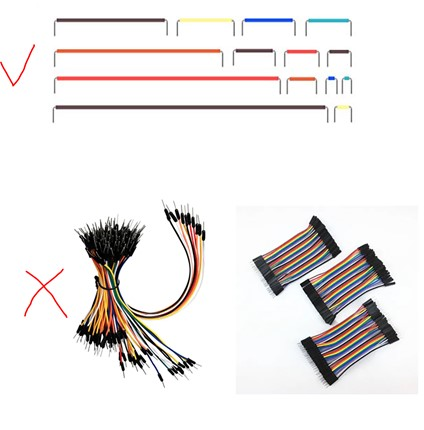
\includegraphics[width=1\textwidth]{wiring.jpg}
	\caption{Example of what the wires you use should look like.} \label{fig:wires}
\end{figure}

%%%%%%%%%%%%%%%%%%%%%%%%%%%%%%%%%%%%%%%%%%%%%%%%%%%%%%%%%%%%%%%%%%%%%%%%%%%%%%%%%%%%%%%%%%%%%%%%%%%%%%%
\section{In-Lab Requirements}
%%%%%%%%%%%%%%%%%%%%%%%%%%%%%%%%%%%%%%%%%%%%%%%%%%%%%%%%%%%%%%%%%%%%%%%%%%%%%%%%%%%%%%%%%%%%%%%%%%%%%%%

To be accomplished in lab:

\begin{enumerate}
	\item Pre-lab check
	\item Review of Lab Rules and Policies
	\item Hand out lab kits
	\item Live tutorial
\end{enumerate}

%%%%%%%%%%%%%%%%%%%%%%%%%%%%%%%%%%%%%%%%%%%%%%%%%%%%%%%%%%%%%%%%%%%%%%%%%%%%%%%%%%%%%%%%%%%%%%%%%%%%%%%
\section{Write Up}
%%%%%%%%%%%%%%%%%%%%%%%%%%%%%%%%%%%%%%%%%%%%%%%%%%%%%%%%%%%%%%%%%%%%%%%%%%%%%%%%%%%%%%%%%%%%%%%%%%%%%%%

Typically this section would details the requirements for the write up but there is no write up for this lab. 

%
%\section{Background}
%
%The reference manual for the Analog Discovery 1 can be found \href{https://reference.digilentinc.com/_media/analog_discovery:analog_discovery_rm.pdf}{here} and the reference manual for the Analog Disocver 2 can be found \href{https://reference.digilentinc.com/_media/reference/instrumentation/analog-discovery-2/ad2_rm.pdf}{here}
%
%David Munzer has written a few tutorials for concerning the Digilant Analog Discovery, bread boarding, and debugging. All three presentations can be found on Canvas in the laboratory file folder. Focus on the Digilant Analog Discovery and bread boarding tutorial for the purposes of this lab.
%
%\section{Pre-lab}
%
%Each student must have a working Digilent Analog Discovery and the latest version of Waveforms (Waveforms 2015) installed on their laptop. If you have to choose, the Analog Discovery 2 with a parts kit is preferred. Failure to have an Analog Discovery and/or the software installed on their laptop will result in a zero for the lab and said student will not be allowed to complete the lab.
%
%\section{Experiment}
%
%This experiment will focus on working with the many tools associated with the Analog Discovery. Whenever saving images from Waveforms, traces must be labeled appropriately and the figure must be 
%exported correctly. Screen shots of the Waveforms software, not matter how well cropped will not be accepted.
%
%\begin{figure}[h] 
	%\centering
	%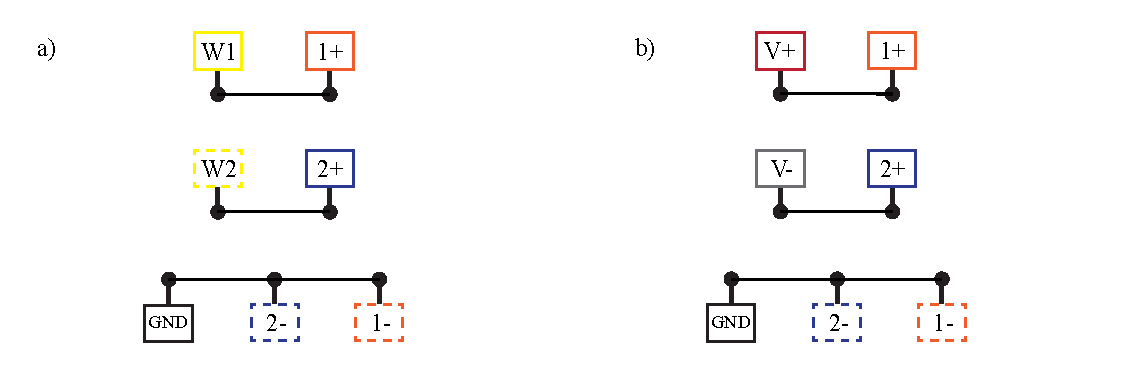
\includegraphics[width=1\textwidth]{Lab1-WavegenScopeConnections.pdf}
	%\caption{Circuit diagram for connecting the wavegen outputs to the scope probes (a) and connection the power supplies to the scope probes (b). Note that the scope probe negative terminals, indicated with a dashed line in the diagram and a white strip on the Analog Discovery wire, must be tied to the Analog Discovery ground. Also, the negative power supply wire is white on the Analog Discovery and has been indicated by gray box in the Figure. } \label{fig:WavegenScopeConnections}
%\end{figure}
%
%
%\begin{enumerate}
	%\item Use the Wavegen to generate a 10 kHz sine wave with an amplitude of 2 V, an offset of 0 V, a symmetry of 50\% and a phase of 0 degrees. Connect the output of the Wavegen on the Analog Discovery to the scope probes and measure the results using the Scope tool as shown in \hyperref[fig:WavegenScopeConnections]{Figure \ref*{fig:WavegenScopeConnections} (a)} and choose an appropriate time base and voltage range; display at least one period but no more than three periods.
	%\item Label the sine wave appropriately and then export an image of the Scope screen. Go to \textbf{File} -> \textbf{Export} and then set the \textbf{Source} to \textbf{Acquisition}. Click save and then choose an appropriate name and location for file. For the lab check, images must be shown to the lab instructor for accuracy. \label{itm:singlesine}
	%\item Using the same signal on channel 1, generate a second sine wave on channel 2 in the Wavegen that is 180 degrees out of phase. Remember to wire up the second Wavegen and Scope channels. 
	%\item On the scope, display channel 1, 2, and add a simple math channel that plots Channel 1 - Channel 2. Again, choose the appropriate time, voltage scales, and label the traces appropriately. Save an image of the Scope acquisition. \label{itm:dualsine}
	%\item Wire up the Analog Discovery so that the variable power supplies on the Analog Discovery are connected to the scope probes as shown in \hyperref[fig:WavegenScopeConnections]{Figure \ref*{fig:WavegenScopeConnections} (b)}. Set the power supplies to +5 V and -5 V (Analog Discovery 1 is fixed at +/-5 V while the Analog Discovery 2 has variable supplies). Display the results on the Scope and save an image with the appropriate labels and voltage scale. \label{itm:voltagerefs}
	%\item Reconnect the Wavegen to the scope probes as shown in \hyperref[fig:WavegenScopeConnections]{Figure \ref*{fig:WavegenScopeConnections} (a)} and generate a 100 kHz square wave with a 1 V amplitude, 1 V offset, symmetry of 50\%, 0 degree phase offset. Choose a time base that displays at least 1 period but no more than 3 periods. Also, set the trigger level so that the trace does not ``run''. Save an image of the acquisition. \label{itm:squarewave}
	%\item Add two X cursors, \textbf{View} -> \textbf{Cursors} -> X \textbf{Cursors}, and confirm that the period corresponds to a 100 kHz signal. Similarly, add two Y cursors and confirm that the peak-to-peak voltage is 2 V. Save an image of the scope showing the X and Y cursors (set the source to Scope instead of Acquisition). \label{itm:cursors}
%\end{enumerate}
%
%\section{Discussion Questions}
%
%Typically this would be where the discussion quires are located associated with the lab but for lab 1 there is no report and therefore no discussion questions.
%
%\section{Lab Check}
%
%All students must check out of the lab and the lab instructor the following items. Usually they are images from the lab, tables of values, completed circuits, etc..
%
%\begin{enumerate}
	%\item \hyperref[itm:singlesine]{Item \ref*{itm:singlesine}} - Single sine wave plot.
	%\item \hyperref[itm:dualsine]{Item \ref*{itm:dualsine}} - Dual sine wave plot.
	%\item \hyperref[itm:voltagerefs]{Item \ref*{itm:voltagerefs}} - Reference voltages plot.
	%\item \hyperref[itm:squarewave]{Item \ref*{itm:squarewave}} - Square wave plot.
	%\item \hyperref[itm:cursors]{Item \ref*{itm:cursors}} -  Square wave with cursors plot.
%\end{enumerate}
%
%\section{Lab Practical Exam}
%
%Once the lab check is completed you can complete the lab practical exam. The lab instructor will ask you to generate and display a variety of signals. The exam is pass or fail and it can be repeated as many times as necessary until the lab session ends. 
%

\include{Lab2}
\include{Lab3}
\chapter{Lab 4 - Controlled Sources}

%%%%%%%%%%%%%%%%%%%%%%%%%%%%%%%%%%%%%%%%%%%%%%%%%%%%%%%%%%%%%%%%%%%%%%%%%%%%%%%%%%%%%%%%%%%%%%%%%%%%%%%
\section{Objective}
%%%%%%%%%%%%%%%%%%%%%%%%%%%%%%%%%%%%%%%%%%%%%%%%%%%%%%%%%%%%%%%%%%%%%%%%%%%%%%%%%%%%%%%%%%%%%%%%%%%%%%%

The purpose of this lab is gain an understanding of controlled voltage sources and the effects of input resistance, output resistance, and feedback. 

%%%%%%%%%%%%%%%%%%%%%%%%%%%%%%%%%%%%%%%%%%%%%%%%%%%%%%%%%%%%%%%%%%%%%%%%%%%%%%%%%%%%%%%%%%%%%%%%%%%%%%%
\section{Materials}
%%%%%%%%%%%%%%%%%%%%%%%%%%%%%%%%%%%%%%%%%%%%%%%%%%%%%%%%%%%%%%%%%%%%%%%%%%%%%%%%%%%%%%%%%%%%%%%%%%%%%%%

\begin{itemize}
	\item Laptop with LTSpice
\end{itemize}

%%%%%%%%%%%%%%%%%%%%%%%%%%%%%%%%%%%%%%%%%%%%%%%%%%%%%%%%%%%%%%%%%%%%%%%%%%%%%%%%%%%%%%%%%%%%%%%%%%%%%%%
\section{Introduction}
%%%%%%%%%%%%%%%%%%%%%%%%%%%%%%%%%%%%%%%%%%%%%%%%%%%%%%%%%%%%%%%%%%%%%%%%%%%%%%%%%%%%%%%%%%%%%%%%%%%%%%%

A controlled source references a voltage or current and in turn generates a voltage or current, often amplifying the reference in the process. Four possible variations exist: 
	\begin{itemize}
		\item Voltage Controlled Voltage Source (VCVS)
		\item Voltage Controlled Current Source (VCCS)
		\item Current Controlled Voltage Source (CCVS)
		\item Current Controlled Current Source (CCCS)
	\end{itemize}
\noindent For this course, the primary concern is a VCVS because is serves as part of the model for an amplifier. 

\subsection{Voltage Controlled Voltage Source}

As the name implies, a VCVS generates a voltage controlled by a different voltage. Usually this voltage is across a resistance but for the ideal case, the resistance is infinite and appears as an open circuit. Similarly, the output is simply the gain, $A$, multiplied by the control voltage, $V_i$, when the output resistance is zero and appears as a wire. Consider the models for a VCVS show in \hyperref[fig:4sourcemodel]{Figure \ref*{fig:4sourcemodel} (a) through (c)}. For the ideal case, (a) and (b), the voltage drop $V_i$ provides the control voltage for the controlled source which generates a voltage output of $A V_i$. Practically, the input and output resistances must be considered as shown in (c). 

\begin{figure} [h]
	\centering
		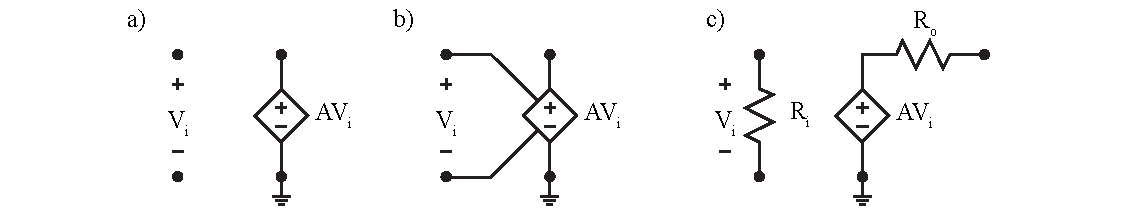
\includegraphics[width=1\textwidth]{Lab4AidealSource.pdf}
	\caption{Representations of a voltage controlled voltage source, ideal model (a), variation used in LTspice (b), and a model with an input and output resistance (c).} \label{fig:4sourcemodel}
\end{figure}


%%%%%%%%%%%%%%%%%%%%%%%%%%%%%%%%%%%%%%%%%%%%%%%%%%%%%%%%%%%%%%%%%%%%%%%%%%%%%%%%%%%%%%%%%%%%%%%%%%%%%%%%
%\subsection{Input and Output Resistance}
%%%%%%%%%%%%%%%%%%%%%%%%%%%%%%%%%%%%%%%%%%%%%%%%%%%%%%%%%%%%%%%%%%%%%%%%%%%%%%%%%%%%%%%%%%%%%%%%%%%%%%%%


%%%%%%%%%%%%%%%%%%%%%%%%%%%%%%%%%%%%%%%%%%%%%%%%%%%%%%%%%%%%%%%%%%%%%%%%%%%%%%%%%%%%%%%%%%%%%%%%%%%%%%%
\subsection{Feedback}
%%%%%%%%%%%%%%%%%%%%%%%%%%%%%%%%%%%%%%%%%%%%%%%%%%%%%%%%%%%%%%%%%%%%%%%%%%%%%%%%%%%%%%%%%%%%%%%%%%%%%%%

%Obviously the gain of the controlled source is the variable most affected by the Monte Carlo simulations but that's expected, the output voltage depends directly on the input voltage multiplied by the gain of the controlled source. While this is not a serious problem for a small gain, 10, it is a serious problem when the gain is large, on the order of $10^5$. 

%Before the advent of modern electronics with better control of the fabrication process, the gain would often vary over a wide range which proved problematic when an exact gain was desired. While convenient to set the model gain of the controlled source to a value of 10, it's not practical, the gain can't be changed after production when a gain of 15 or 1 is desired. Often a large gain would be used in order to amplify small signals but this presents another problem, the input must be small in order to prevent the output from clipping or saturation, beyond the scope of our current mode. The answer to these two problems, high variation in the gain and high gain, is feedback. Feeding back the output signal back to the input allows the overall output to be dependent on external components, resistors, that can be well controlled.

The combination of an amplifier with feedback can be represented many ways. One of the generic ways is a signal flow diagram as shown in \hyperref[fig:4sigflow]{Figure \ref*{fig:4sigflow}}. 

\begin{figure} [h]
	\centering
		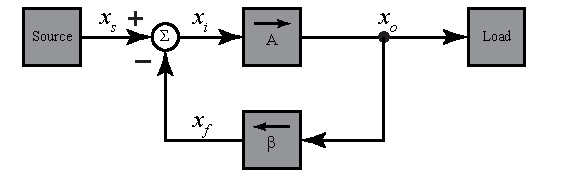
\includegraphics[width=0.5\textwidth]{Lab4signalflow.pdf}
	\caption{A signal flow diagram for an amplifier with feedback. Each voltage is represented by some value $x$, with an amplifier of gain A, and a feedback factor of $\beta$.} \label{fig:4sigflow}
\end{figure}

The amplifier has a gain, A, which is called the open-loop gain and represents the gain from the input, $x_i$, of the amplifier to the output, $x_o$. This is described by the equation

\begin{equation}
	x_o = A x_i
\end{equation}

\noindent In this example, the output is feedback through a feedback network with a feedback factor, $\beta$. Which gives the feedback voltage, $x_f$, equal to the output voltage, $x_o$, times the feedback factor, $\beta$.

\begin{equation}
	x_f = \beta x_o
\end{equation}

\noindent The feedback voltage, $x_f$, is then subtracted from the source signal, $x_s$, which gives the input to the amplifier, $x_i$. 

\begin{equation}
	x_i = x_s - x_f
\end{equation}

\noindent Here it's important to recognize that the loading effects of the load and source have been neglected as this is a generic case with finite gain. The total gain of the system, with feedback, then becomes

\begin{equation}
	A_f \equiv \frac{x_o}{x_s} = \frac{A}{1 + A \beta}
\end{equation}

\noindent This equation represents the closed loop gain of the system which is smaller than the open loop gain by a factor of $1+A\beta$, called the amount of feedback. The quantity A$\beta$ is the loop gain and must be positive. Often the loop gain is large, $A\beta \gg 1$, or simply A is large, which simplifies the closed loop gain to

\begin{equation}
	A_f \simeq \frac{1}{\beta}
\end{equation}

\noindent Which gives a result entirely dependent on the feedback factor. This is an important because if the gain, A, is large, the closed loop gain will depend entirely on elements in the feedback network. 

%%%%%%%%%%%%%%%%%%%%%%%%%%%%%%%%%%%%%%%%%%%%%%%%%%%%%%%%%%%%%%%%%%%%%%%%%%%%%%%%%%%%%%%%%%%%%%%%%%%%%%%
\section{Pre-Lab Requirements}
%%%%%%%%%%%%%%%%%%%%%%%%%%%%%%%%%%%%%%%%%%%%%%%%%%%%%%%%%%%%%%%%%%%%%%%%%%%%%%%%%%%%%%%%%%%%%%%%%%%%%%%

Complete the following using LTspice.

%%%%%%%%%%%%%%%%%%%%%%%%%%%%%%%%%%%%%%%%%%%%%%%%%%%%%%%%%%%%%%%%%%%%%%%%%%%%%%%%%%%%%%%%%%%%%%%%%%%%%%%
\subsection{Simulating a Controlled Source} \label{ssec:4simcs}
%%%%%%%%%%%%%%%%%%%%%%%%%%%%%%%%%%%%%%%%%%%%%%%%%%%%%%%%%%%%%%%%%%%%%%%%%%%%%%%%%%%%%%%%%%%%%%%%%%%%%%%

\begin{figure} [h]
	\centering
		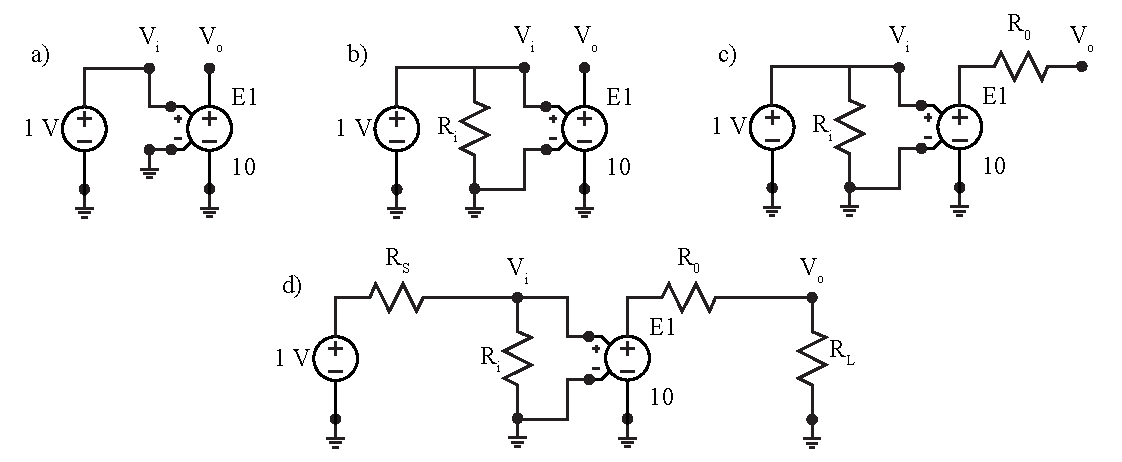
\includegraphics[width=1\textwidth]{Lab4ALTsource.pdf}
	\caption{Different configurations for a VCVS in LTspice: the ideal case (a), with an input resistance (b), with an input resistance and output resistance (c), and with a source and load resistance (d).} \label{fig:4sourcespice}
\end{figure}


\begin{enumerate}
	\item Setup a simple voltage controlled voltage source in LTspice with a gain of 10 as shown in \hyperref[fig:4sourcespice]{Figure \ref*{fig:4sourcespice} (a)}. Use the e component in LTspice, voltage dependent voltage source, and set the gain, E, to 10 and run a DC operating point solution to confirm that the output of the controlled source is 10 V. Table the input, $V_i$, and output, $V_o$, voltages. \label{itm:4ssec1itm1}
	\item Connect an input resistance from the voltage input to ground as shown in \hyperref[fig:4sourcespice]{Figure \ref*{fig:4sourcespice} (b)}. Set the resistance to 10 k$\Omega$ and re-run the DC operating point simulation, table the values for $V_i$ and $V_o$.
	\item Connect an output resistance form the controlled source output as shown in \hyperref[fig:4sourcespice]{Figure \ref*{fig:4sourcespice} (c)}. Set the resistance to 10 k$\Omega$ and re-run the DC operating point simulation, table the values for $V_i$ and $V_o$.
	\item Connect the circuit as shown in \hyperref[fig:4sourcespice]{Figure \ref*{fig:4sourcespice} (d)} with a source, $R_S$, and load, $R_L$, resistance. Set both values to 50 $\Omega$ and re-run the DC operating point simulation, table the values for $V_i$ and $V_o$. \label{itm:4ssec1itm4}
	\item Step through different values of $R_i$ from 0.1 to 1Meg in powers of 10 and determine the best value for the input resistance. Plot the input voltage, $V_i$, on a log scale and save an image of the plot and circuit. \label{itm:4ssec1itm5}
	\item Using the value of $R_i$ from the previous step, step through different values of $R_o$ from 0.1 to 1Meg in powers of 10 and determine the best value for the output resistance. Plot the output voltage, $V_o$, on a log scale and save an image of the plot and circuit. \label{itm:4ssec1itm6}
\end{enumerate}

%%%%%%%%%%%%%%%%%%%%%%%%%%%%%%%%%%%%%%%%%%%%%%%%%%%%%%%%%%%%%%%%%%%%%%%%%%%%%%%%%%%%%%%%%%%%%%%%%%%%%%%
\subsection{Monte Carlo Simulations} \label{ssec:4MonteCarlo}
%%%%%%%%%%%%%%%%%%%%%%%%%%%%%%%%%%%%%%%%%%%%%%%%%%%%%%%%%%%%%%%%%%%%%%%%%%%%%%%%%%%%%%%%%%%%%%%%%%%%%%%

\begin{figure} [h]
	\centering
		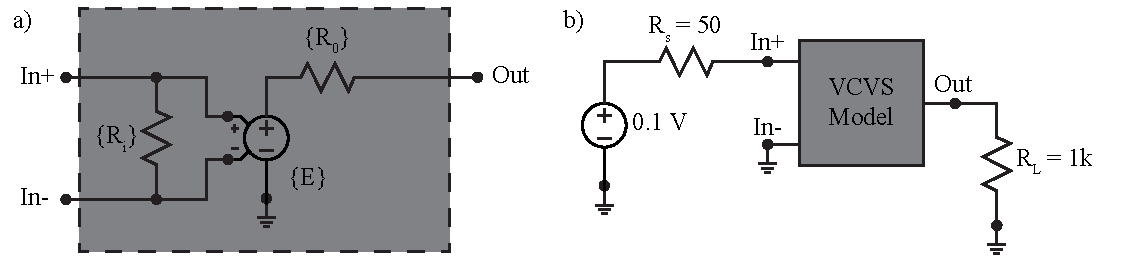
\includegraphics[width=1\textwidth]{Lab4Agenmodel.pdf}
	\caption{A general model for a voltage controlled voltage source with input and output resistance (a) and model used in conjunction with a DC source and a source and load resistance (b). Note that each of the values for the two resistors and the gain are LTspice variables, denoted by the curly brackets, \{\}.} \label{fig:4genmod}
\end{figure}

\begin{enumerate}
	\item Create a sub-circuit of the VCVS from \hyperref[ssec:4simcs]{Subsection \ref*{ssec:4simcs}} as shown in \hyperref[fig:4genmod]{Figure \ref*{fig:4genmod} (a)}. Set the input resistance and output resistance to the previously determined values and the gain to 10. The second half of this video, \url{http://www.linear.com/solutions/7723}, is a helpful tutorial for creating a sub-circuit (symbol) from an already created circuit. Note that default parameters are defined in the subcircuit. To quickly make a subcircuit, in LTspice navigate to the Hierarchy tab, and select "Open this sheet's symbol". This will prompt you to generate a new symbol file, select yes. You can now access this symbol file under the component selection option. All you need to do is change the top directory (the drop down list at the top of the page). Your top directory will be wherever on your computer you created your original LTspice .asc file, and the symbol file will have been generated and must remain in that same directory/folder.
	\item Connect a 0.1V DC voltage source in series with a source resistance of 50 $\Omega$ to the positive input terminal, connect the negative input terminal to ground, and a 1k $\Omega$ resistor to ground at the output as shown in \hyperref[fig:4genmod]{Figure \ref*{fig:4genmod} (b)}.
	\item Run a Monte Carlo simulation for the gain, E, of the VCVS. Set the tolerance to 0.1 (10\%) and run the simulation for 1000 iterations. The Monte Carlo function call can be passed in as a variable to the VCVS model where E = \{mc\{10,tol\}\} in the Value field for the Value attribute. Plot the output voltage and save an image of the circuit and plot. \label{itm:4ssec2itm3}
	\item Repeat the Monte Carlo simulation for the input resistance, Ri. Save an image of the output voltage plot. \label{itm:4ssec2itm4}
	\item Repeat the Monte Carlo simulation for the output resistance, Ro. Save an image of the output voltage plot. \label{itm:4ssec2itm5}
\end{enumerate}

%%%%%%%%%%%%%%%%%%%%%%%%%%%%%%%%%%%%%%%%%%%%%%%%%%%%%%%%%%%%%%%%%%%%%%%%%%%%%%%%%%%%%%%%%%%%%%%%%%%%%%%
\subsection{Feedback} \label{ssec:4Feedback}
%%%%%%%%%%%%%%%%%%%%%%%%%%%%%%%%%%%%%%%%%%%%%%%%%%%%%%%%%%%%%%%%%%%%%%%%%%%%%%%%%%%%%%%%%%%%%%%%%%%%%%%

The VCVS model developed in previous sections has been re-drawn using the more common symbol for an amplifier as shown in \hyperref[fig:4feedbackcombo]{Figure \ref*{fig:4feedbackcombo} (a)}. However, the model is still the same and it's not required to redraw your model. 

\begin{figure} [h]
	\centering
		\includegraphics[width=1\textwidth]{Lab4AvcvsTri.pdf}
	\caption{The VSCS model redrawn as the more common amplifier model symbol (a), unity gain configuration (b), and non-inverting gain configuration (c).} \label{fig:4feedbackcombo}
\end{figure}

\begin{enumerate}
	\item Construct the circuit as shown in \hyperref[fig:4feedbackcombo]{Figure \ref*{fig:4feedbackcombo} (b)}. The resistors $R_S$ and $R_L$ remain 50 $\Omega$ and 1 k$\Omega$ respectively. 
	%\item Calculate the ideal gain, with and without finite gain, for this circuit, \hyperref[fig:4feedbackcombo]{Figure \ref*{fig:4feedbackcombo} (b)}. Assume the input resistance is infinite, the gain is infinite and finite, $10\times10^5$, and the output resistance is zero. \label{itm:4ssec3itm2}
	\item Run a Monte Carlo simulation for the gain, E, of the VSVS model. Set the gain to 10E5, tolerance to 0.3 (30\%), and run the simulation for 1000 iterations. Plot the output voltage and save an image of the circuit and plot. \label{itm:4ssec3itm3}
	\item Construct the circuit as shown in \hyperref[fig:4feedbackcombo]{Figure \ref*{fig:4feedbackcombo} (c)}. Set $R_2$ to 2 k$\Omega$ and $R_1$ to 1 k$\Omega$. The resistors $R_S$ and $R_L$ remain 50 $\Omega$ and 1 k$\Omega$ respectively. 
	%\item Calculate the ideal gain, with and without finite gain, for this circuit, \hyperref[fig:4feedbackcombo]{Figure \ref*{fig:4feedbackcombo} (c)}. Assume the input resistance is infinite, the gain is infinite and finite, $10\times10^5$, and the output resistance is zero. \label{itm:4ssec3itm5}
	\item Run a Monte Carlo simulation for the gain, E, of the VSVS model. Set the gain to 10E5, tolerance to 0.3 (30\%), and run the simulation for 1000 iterations. Plot the output voltage and save an image of the circuit and plot. \label{itm:4ssec3itm6}
\end{enumerate} 

%%%%%%%%%%%%%%%%%%%%%%%%%%%%%%%%%%%%%%%%%%%%%%%%%%%%%%%%%%%%%%%%%%%%%%%%%%%%%%%%%%%%%%%%%%%%%%%%%%%%%%%
\section{In-Lab Requirements}
%%%%%%%%%%%%%%%%%%%%%%%%%%%%%%%%%%%%%%%%%%%%%%%%%%%%%%%%%%%%%%%%%%%%%%%%%%%%%%%%%%%%%%%%%%%%%%%%%%%%%%%

The following must be completed and submitted to Canvas before the start of lab. 

\begin{enumerate}
	\item \hyperref[ssec:4simcs]{Subsection \ref*{ssec:4simcs}}:
		\begin{enumerate}
			\item Items \hyperref[itm:4ssec1itm1]{\ref*{itm:4ssec1itm1}} - \hyperref[itm:4ssec1itm1]{\ref*{itm:4ssec1itm4}}: Table of input and output voltages. 
			\item \hyperref[itm:4ssec1itm5]{Item \ref*{itm:4ssec1itm5}}: Image of circuit and plot of the input voltage.
			\item \hyperref[itm:4ssec1itm6]{Item \ref*{itm:4ssec1itm6}}: Image of circuit and plot of the output voltage.
		\end{enumerate}
	\item \hyperref[{ssec:4MonteCarlo}]{Subsection \ref*{ssec:4MonteCarlo}}:
		\begin{enumerate}
			\item \hyperref[itm:4ssec2itm3]{Item \ref*{itm:4ssec2itm3}}: Image of circuit and plot of the output voltage.
			\item \hyperref[itm:4ssec2itm4]{Item \ref*{itm:4ssec2itm4}}: Plot of the output voltage.
			\item \hyperref[itm:4ssec2itm5]{Item \ref*{itm:4ssec2itm5}}: Plot of the output voltage.
		\end{enumerate}
	\item \hyperref[ssec:4Feedback]{Subsection \ref*{ssec:4Feedback}}:
		\begin{enumerate}
			%\item \hyperref[itm:4ssec3itm2]{Item \ref*{itm:4ssec3itm2}}: Ideal gain.
			\item \hyperref[itm:4ssec3itm3]{Item \ref*{itm:4ssec3itm3}}: Image of circuit and plot of the output voltage.
			%\item \hyperref[itm:4ssec3itm5]{Item \ref*{itm:4ssec3itm5}}: Ideal gain. 
			\item \hyperref[itm:4ssec3itm6]{Item \ref*{itm:4ssec3itm6}}: Image of circuit and plot of the output voltage.
		\end{enumerate}
\end{enumerate}

Complete the following items in lab.

%%%%%%%%%%%%%%%%%%%%%%%%%%%%%%%%%%%%%%%%%%%%%%%%%%%%%%%%%%%%%%%%%%%%%%%%%%%%%%%%%%%%%%%%%%%%%%%%%%%%%%%
\subsection{Worst Case Analysis} \label{ssec:4worstcase}
%%%%%%%%%%%%%%%%%%%%%%%%%%%%%%%%%%%%%%%%%%%%%%%%%%%%%%%%%%%%%%%%%%%%%%%%%%%%%%%%%%%%%%%%%%%%%%%%%%%%%%%

While Monte Carlo analysis is useful for looking at a range of possible values, often times it's important to see the potential worst case values given a specified tolerance. Use the VCVS model that was previusly devloped with the values of $R_i$ and $R_o$ previously defined and a gain of 10E5. 

\begin{figure} [h]
	\centering
		\includegraphics[width=1\textwidth]{Lab4wc.pdf}
	\caption{Non-inverting configuration with the necessary resistor values for a worst case simulation (a) and inverting configuration with the necessary resistor values for a worst case simulation (b).} \label{fig:4wcckts}
\end{figure}


\begin{enumerate}
	\item Construct the circuit as shown in \hyperref[fig:4wcckts]{Figure \ref*{fig:4wcckts} (a)}
	\item Run a DC operating point simulation with the following additional parameters:
\begingroup
    \fontsize{10pt}{12pt}\selectfont
	\begin{verbatim}
		.func binary(run,index) floor(run/(2**index))-2*floor(run/(2**(index+1)))
		.func wc(nom,tol,index) if(run==numruns,nom,if(binary(run,index),nom*(1+tol),nom*(1-tol)))
		.param numruns=4
		.step param run 0 4 1
		.param tol=0.05
	\end{verbatim}
\endgroup

	\item Plot the output voltage and save an image of the plot. Determine the worst case results, which resistor tolerances, that gives the highest and lowest output voltages. \label{itm:4ssec4itm3}
	\item Repeat the simulation for a tolerance of 0.01 (1\%), 0.005 (0.5\%), 0.001 (0.1\%), 0.0005 (0.05\%), and 0.0001 (0.01\%). For each case, table the high, low output voltages, and determine the cost of the components. Use the following Digikey link to determine pricing: \url{http://digikey.com}. Search through hole resistors, select the ones in-stock for 0.25 Watt, Carbon Film according to the required tolerance.  \label{itm:4ssec4itm4}
	\item Construct the circuit as shown in \hyperref[fig:4wcckts]{Figure \ref*{fig:4wcckts} (b)}
	\item Run a DC operating point simulation with the parameters previously stated.
	\item Plot the output voltage and save an image of the plot. Determine the worst case results that gives the highest and lowest output voltages. \label{itm:4ssec4itm7}
	\item Repeat the simulation for a tolerance of 0.01 (1\%), 0.005 (0.5\%), 0.001 (0.1\%), 0.0005 (0.05\%), and 0.0001 (0.01\%). For each case, table the high, low output voltages, and determine the cost of the components. \label{itm:4ssec4itm8}
\end{enumerate}

%%%%%%%%%%%%%%%%%%%%%%%%%%%%%%%%%%%%%%%%%%%%%%%%%%%%%%%%%%%%%%%%%%%%%%%%%%%%%%%%%%%%%%%%%%%%%%%%%%%%%%%
\section{Write Up}
%%%%%%%%%%%%%%%%%%%%%%%%%%%%%%%%%%%%%%%%%%%%%%%%%%%%%%%%%%%%%%%%%%%%%%%%%%%%%%%%%%%%%%%%%%%%%%%%%%%%%%%

Include the following in the write up.

\begin{enumerate}
	\item \hyperref[ssec:4worstcase]{Subsection \ref*{ssec:4worstcase}}
		\begin{enumerate}
			\item \hyperref[itm:4ssec4itm3]{Item \ref*{itm:4ssec4itm3}}: Output voltage plot for a 5\% tolerance and the highest and lowest output voltage cases. 
			\item \hyperref[itm:4ssec4itm4]{Item \ref*{itm:4ssec4itm4}}: Tabled output voltage range and pricing for different resistor tolerances. 
			\item \hyperref[itm:4ssec4itm7]{Item \ref*{itm:4ssec4itm7}}: Output voltage plot for a 5\% tolerance and the highest and lowest output voltage cases. 
			\item \hyperref[itm:4ssec4itm8]{Item \ref*{itm:4ssec4itm8}}: Tabled output voltage range and pricing for different resistor tolerances. 
		\end{enumerate}
\end{enumerate}

Discuss the benefits of feedback, worst case analysis for different resistor tolerances, and the cost/benefit trade off for different resistor tolerances.

For all lab write up submissions and reports the backgrounds for LTSpice and Waveforms should be changed from dark background to light background to make them readable for grading. 

If the prelab simulation is incorrect, do not compare the in lab results to wrong values.  Correct numbers or circuit schematics should be used in the write-up report.


\chapter{Lab 5 - Operational Amplifiers}

%%%%%%%%%%%%%%%%%%%%%%%%%%%%%%%%%%%%%%%%%%%%%%%%%%%%%%%%%%%%%%%%%%%%%%%%%%%%%%%%%%%%%%%%%%%%%%%%%%%%%%%
\section{Objective}
%%%%%%%%%%%%%%%%%%%%%%%%%%%%%%%%%%%%%%%%%%%%%%%%%%%%%%%%%%%%%%%%%%%%%%%%%%%%%%%%%%%%%%%%%%%%%%%%%%%%%%%

The purpose of this lab is to introduce  operational amplifiers through the ideal op amp model, spice op amp model, and practical applications of op amps in common configurations. 

%%%%%%%%%%%%%%%%%%%%%%%%%%%%%%%%%%%%%%%%%%%%%%%%%%%%%%%%%%%%%%%%%%%%%%%%%%%%%%%%%%%%%%%%%%%%%%%%%%%%%%%
\section{Materials}
%%%%%%%%%%%%%%%%%%%%%%%%%%%%%%%%%%%%%%%%%%%%%%%%%%%%%%%%%%%%%%%%%%%%%%%%%%%%%%%%%%%%%%%%%%%%%%%%%%%%%%%

\begin{itemize}
	\item Laptop with LTSpice
	\item Analog Discovery
	\item Breadboard
	\item Wiring kit
	\item Lab parts kit with TLV272
\end{itemize}

%%%%%%%%%%%%%%%%%%%%%%%%%%%%%%%%%%%%%%%%%%%%%%%%%%%%%%%%%%%%%%%%%%%%%%%%%%%%%%%%%%%%%%%%%%%%%%%%%%%%%%%
\section{Introduction}
%%%%%%%%%%%%%%%%%%%%%%%%%%%%%%%%%%%%%%%%%%%%%%%%%%%%%%%%%%%%%%%%%%%%%%%%%%%%%%%%%%%%%%%%%%%%%%%%%%%%%%%

There is a large variety of op amp and specialized amplifiers. For this lab the more recent TLV272 is used, a dual op amp, which contains two op amps, or channels, in a single chip.

%%%%%%%%%%%%%%%%%%%%%%%%%%%%%%%%%%%%%%%%%%%%%%%%%%%%%%%%%%%%%%%%%%%%%%%%%%%%%%%%%%%%%%%%%%%%%%%%%%%%%%
\subsection{The Ideal Op Amp}
%%%%%%%%%%%%%%%%%%%%%%%%%%%%%%%%%%%%%%%%%%%%%%%%%%%%%%%%%%%%%%%%%%%%%%%%%%%%%%%%%%%%%%%%%%%%%%%%%%%%%%

Recall that an ideal op amp will have the following properties. 

\begin{itemize}
	\item Zero input current, often called the input bias current and represented as $\mathrm{I_B}$ or $\mathrm{I_{IB}}$. 
	\item Zero input offset voltage, represented as either $\mathrm{V_{IO}}$ or $\mathrm{V_{OS}}$.
	\item Infinite input resistance, represented as $\mathrm{R_{in}}$ or $\mathrm{r_i}$.  
	\item Zero output resistance, represented as $\mathrm{R_{out}}$ or $\mathrm{r_o}$.
	\item Infinite gain, represented as A or $\alpha$ and often called the open loop gain.
\end{itemize}

\noindent These quantities are represented in \hyperref[fig:IdealAmp]{Figure \ref*{fig:IdealAmp}}.

\begin{figure}[h]
	\centering
		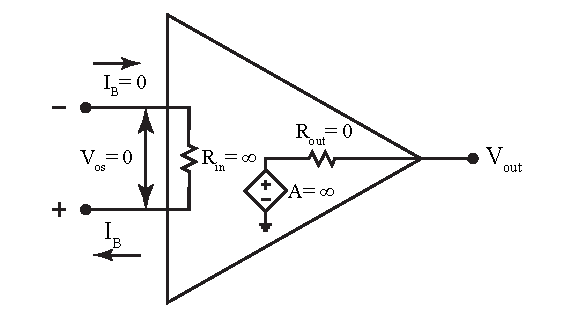
\includegraphics[width=0.5\textwidth]{Lab4idealOpAmp.pdf}
	\caption{Basic op amp model.} \label{fig:IdealAmp}
\end{figure}

However, as should be expected, practical op amp do not have these ideal quantities. For example, the Texas Instrument's TLV272 has finite values for all of the ideal properties. Note that these values vary and depend on productions variation, temperature, and supply voltage.

\begin{itemize}
	\item Finite input bias current, typically 1 pA.
	\item Finite input offset voltage, typically 0.5 mV.
	\item Finite input resistance, typically 1,000 G$\Omega$ differential input resistance.
	\item Finite gain, typically 115 dB (563k)
\end{itemize}

%%%%%%%%%%%%%%%%%%%%%%%%%%%%%%%%%%%%%%%%%%%%%%%%%%%%%%%%%%%%%%%%%%%%%%%%%%%%%%%%%%%%%%%%%%%%%%%%%%%%%%
\subsection{Common Configurations}
%%%%%%%%%%%%%%%%%%%%%%%%%%%%%%%%%%%%%%%%%%%%%%%%%%%%%%%%%%%%%%%%%%%%%%%%%%%%%%%%%%%%%%%%%%%%%%%%%%%%%%

There are a variety of configurations op amps can be used for but there are a few common configurations that form the basis of more complicated op amp circuits. 

\begin{figure} [h]
	\centering
		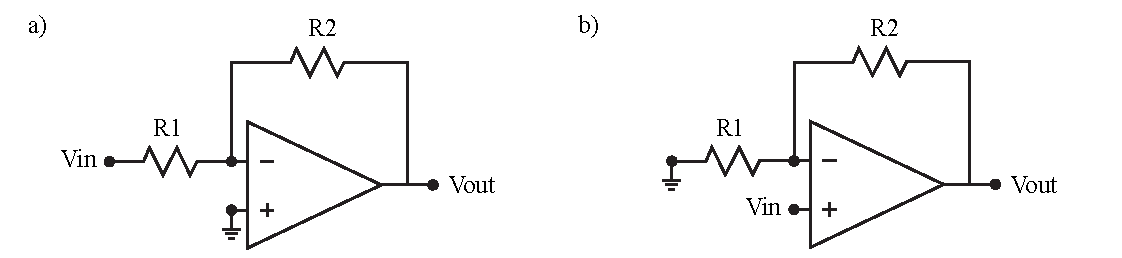
\includegraphics[width=1\textwidth]{Lab4configs.pdf}
	\caption{Different op amp configurations: inverting amplifier (a) and non-inverting amplifier (b)} \label{fig:OAconfigs}
\end{figure}

%%%%%%%%%%%%%%%%%%%%%%%%%%%%%%%%%%%%%%%%%%%%%%%%%%%%%%%%%%%%%%%%%%%%%%%%%%%%%%%%%%%%%%%%%%%%%%%%%%%%%%
\subsubsection{Inverting Amplifier}
%%%%%%%%%%%%%%%%%%%%%%%%%%%%%%%%%%%%%%%%%%%%%%%%%%%%%%%%%%%%%%%%%%%%%%%%%%%%%%%%%%%%%%%%%%%%%%%%%%%%%%

An inverting configuration, \hyperref[fig:OAconfigs]{Fiugre \ref*{fig:OAconfigs} (a)}, takes its name from the inversion that happens from input to output, giving a output voltage proportional to $R_2$ and $R_1$ independent of the actual op amp properties.

\begin{equation}
	\centering
	V_{out} =-\frac{R_2}{R_1}V_{in}
\end{equation}


%%%%%%%%%%%%%%%%%%%%%%%%%%%%%%%%%%%%%%%%%%%%%%%%%%%%%%%%%%%%%%%%%%%%%%%%%%%%%%%%%%%%%%%%%%%%%%%%%%%%%%
\subsubsection{Non-Inverting Amplifier}
%%%%%%%%%%%%%%%%%%%%%%%%%%%%%%%%%%%%%%%%%%%%%%%%%%%%%%%%%%%%%%%%%%%%%%%%%%%%%%%%%%%%%%%%%%%%%%%%%%%%%%

Similar to the inverting case, \hyperref[fig:OAconfigs]{Fiugre \ref*{fig:OAconfigs} (b)}, this configuration results in an output voltage proportional to R2 and R1 but without an inversion and always has a gain of at least 1.

\begin{equation}
	\centering
	V_{out} =(1+\frac{R_2}{R_1})V_{in}
\end{equation}

There is also a special case of the non-inverting amplifier where it is connected as a voltage follower or unity gain amplifier a show in \hyperref[fig:OAbuffer]{Figure \ref*{fig:OAbuffer}}.

\begin{figure} [h]
	\centering
		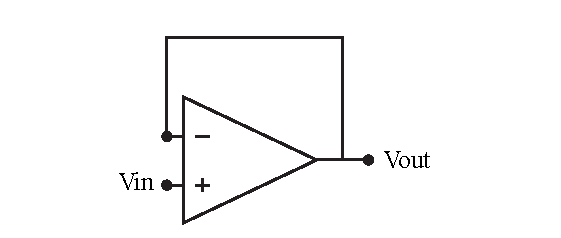
\includegraphics[width=0.5\textwidth]{Lab4buffer.pdf}
	\caption{A non-inverting amplifier configured as a unity gain buffer.} \label{fig:OAbuffer}
\end{figure}

The output is related directly to the input where

\begin{equation}
	\centering
	V_{out} = V_{in}
\end{equation}

\noindent and while this configuration may seem redundant, it has the advantage of providing a large input impedance to the source, $\mathrm{V_{in}}$, and a small output impedance to the load, $\mathrm{V_{out}}$. 

%%%%%%%%%%%%%%%%%%%%%%%%%%%%%%%%%%%%%%%%%%%%%%%%%%%%%%%%%%%%%%%%%%%%%%%%%%%%%%%%%%%%%%%%%%%%%%%%%%%%%%%
%\subsubsection{Summing Amplifier}
%%%%%%%%%%%%%%%%%%%%%%%%%%%%%%%%%%%%%%%%%%%%%%%%%%%%%%%%%%%%%%%%%%%%%%%%%%%%%%%%%%%%%%%%%%%%%%%%%%%%%%%
%
%A summing amplifier, \hyperref[fig:OAconfigs]{Fiugre \ref*{fig:OAconfigs} (c)}, is effectively the same configuration as an inverting amplifier but has multiple inputs that allow for a weighted output voltage. 
%
%\begin{equation}
	%\centering
	%V_{out} = -(\frac{R_4}{R_1}V_1 + \frac{R_4}{R_2}V_2 + \frac{R_4}{R_3}V_3)
%\end{equation}
%
%\noindent When the resistors $R_1$, $R_2$, $R_3$, and $R_4$ are all equal, the output voltage is an equal combination of the input voltages but the resistors can be chosen to weight the input voltages different based on the applicaiton. 
%
%
%%%%%%%%%%%%%%%%%%%%%%%%%%%%%%%%%%%%%%%%%%%%%%%%%%%%%%%%%%%%%%%%%%%%%%%%%%%%%%%%%%%%%%%%%%%%%%%%%%%%%%%
%\subsubsection{Difference Amplifier}
%%%%%%%%%%%%%%%%%%%%%%%%%%%%%%%%%%%%%%%%%%%%%%%%%%%%%%%%%%%%%%%%%%%%%%%%%%%%%%%%%%%%%%%%%%%%%%%%%%%%%%%
%
%Difference amplifiers, \hyperref[fig:OAconfigs]{Figure \ref*{fig:OAconfigs} (d)}, as the name implies takes the difference between the two input voltages resulting in that depends on the ratios of resistor values.
%
%\begin{equation}
	%\centering
	%V_{out} =  V_1 \left(\frac{R_2}{R_1+R_2}\right)\left(\frac{R_3+R_4}{R_3}\right)-V_2\frac{R_4}{R_3}  
%\end{equation}
%
%\noindent When the resistors $R_1 = R_3$ and $R_2 = R_4$ the output voltage simplifies to 
%
%\begin{equation}
	%\centering
	%V_{out} =  (V_1-V_2)\frac{R_2}{R_1}  
%\end{equation}

%%%%%%%%%%%%%%%%%%%%%%%%%%%%%%%%%%%%%%%%%%%%%%%%%%%%%%%%%%%%%%%%%%%%%%%%%%%%%%%%%%%%%%%%%%%%%%%%%%%%%%
\subsection{Op Amp Pins}
%%%%%%%%%%%%%%%%%%%%%%%%%%%%%%%%%%%%%%%%%%%%%%%%%%%%%%%%%%%%%%%%%%%%%%%%%%%%%%%%%%%%%%%%%%%%%%%%%%%%%%

A pinout is a connection diagram for an integrated circuit and shows which pins connect to which op amp terminals internally, not to be confused with the pins in a spice simulation. Op amps have a fairly common pinout resulting in chips that can be swapped out easily. \hyperref[fig:pinout]{Figure \ref*{fig:pinout}} shows the pinout for the TLV272 with the op amp diagram drawn within. 

\begin{figure} [h]
	\centering
		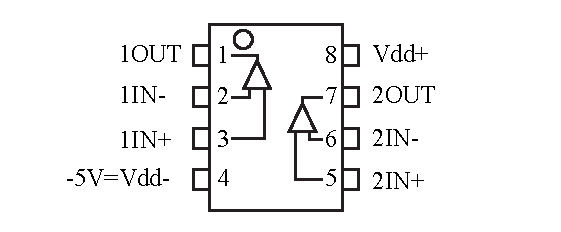
\includegraphics[width=0.5\textwidth]{Lab5pinout.pdf}
	\caption{Pinout for TI's TLV272. Note that two op amps are contained, often called a dual op amp, within a single chip.} \label{fig:pinout}
\end{figure}


\begin{table}[h]
\begin{center}
\begin{tabular}{|l|l|l|}
	\hline
	\textbf{Name} & \textbf{Number} & \textbf{Description} \\ \hline
	1OUT & 1 & Output of the first op amp \\ \hline
	1IN- & 2 & Inverting input of the first op amp \\ \hline
	1IN+ & 3 & Non-inverting input of the first op amp \\ \hline
	Vdd- & 4 & Negative supply, connected to ground for single supply operation \\ \hline
	2IN+ & 5 & Non-inverting input of the second op amp \\ \hline
	2IN- & 6 & Inverting input of the second op amp \\ \hline
	2OUT & 7 & Output of the second op amp \\ \hline
	Vdd+ & 8 & Positive supply \\ 
	\hline 
\end{tabular}
\end{center}
\caption{Pin descriptions from the TLV272 datasheet.}
\label{tbl:TLV272pinout}
\end{table}


The pins are numbered from 1 to 8 and count counter-clockwise starting in the upper left and the individual pin descriptions are in \hyperref[tbl:TLV272pinout]{Table \ref*{tbl:TLV272pinout}}. Most of the pins should be familiar from class.

Polarity or the orientation of the chip is determined by a circle or indentation on the chip itself, the TLV272 has a small circle indentation in the upper left hand corner to indicate polarity and the position of pin 1. 

%%%%%%%%%%%%%%%%%%%%%%%%%%%%%%%%%%%%%%%%%%%%%%%%%%%%%%%%%%%%%%%%%%%%%%%%%%%%%%%%%%%%%%%%%%%%%%%%%%%%%%%
%\subsection{Potentiometers}
%%%%%%%%%%%%%%%%%%%%%%%%%%%%%%%%%%%%%%%%%%%%%%%%%%%%%%%%%%%%%%%%%%%%%%%%%%%%%%%%%%%%%%%%%%%%%%%%%%%%%%%
%
%A potentiometer (or ``pot'') is a three terminal resistor as shown in \hyperref[fig:potcktdia]{Figure \ref*{fig:potcktdia}}. The resistance between terminals 1 and 3 is fixed and is equal to the rated value for the potentiometer. Terminal 2 is connected to a movable contact called the arm or wiper and the resistance between terminals 2 and 1 or between 2 and 3 can be varied by moving the arm. If terminals 1 and 3 are connected across a voltage source, then the voltage between terminals 2 and 1 or between 2 and 3 can be varied by moving the arm. In some cases, terminal 2 is connected to either terminal 1 or 3 so that the resistance from terminals 1 to 3 can be varied. 
%
%\begin{figure}[h] 
	%\centering
	%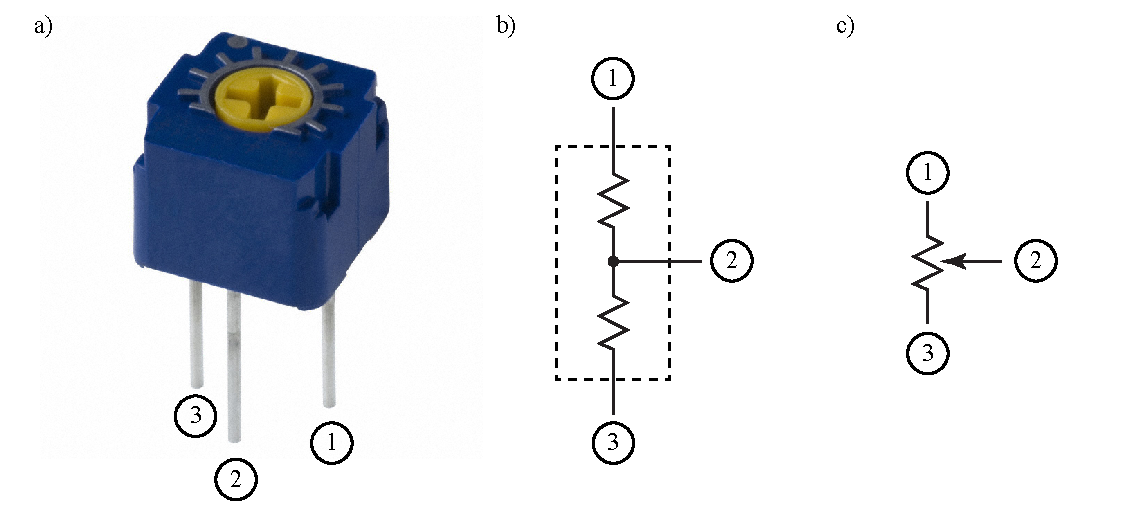
\includegraphics[width=1\textwidth]{lab2potdia.pdf}
	%\caption{A picture of a practical potentiometer with the appropriate pins labeled (a), an equivalent circuit diagram of a potentiometer with the wiper in a fixed position (b), and the common circuit schematic representation for a potentiometer (c).} \label{fig:potcktdia}
%\end{figure}

%%%%%%%%%%%%%%%%%%%%%%%%%%%%%%%%%%%%%%%%%%%%%%%%%%%%%%%%%%%%%%%%%%%%%%%%%%%%%%%%%%%%%%%%%%%%%%%%%%%%%%%
\section{Big Picture}
%%%%%%%%%%%%%%%%%%%%%%%%%%%%%%%%%%%%%%%%%%%%%%%%%%%%%%%%%%%%%%%%%%%%%%%%%%%%%%%%%%%%%%%%%%%%%%%%%%%%%%%

\begin{figure} [h]
	\centering
		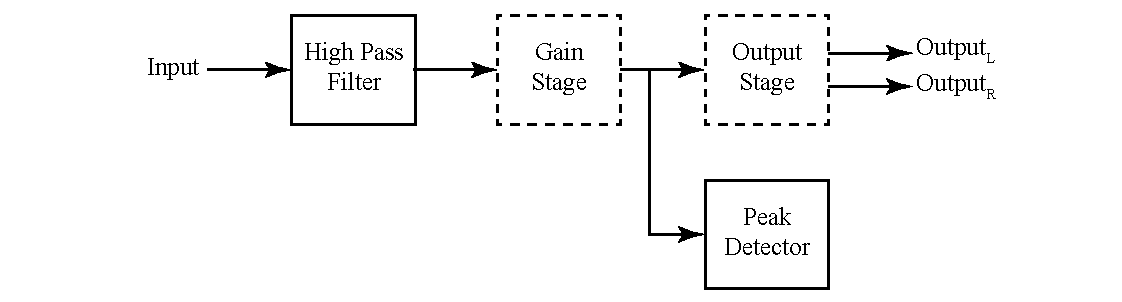
\includegraphics[width=1\textwidth]{Lab5bigpicture.pdf}
	\caption{Big picture with emphasis on the gain and output stages.} \label{fig:5bp}
\end{figure}

This lab focuses on op amps which will be used in the gain and outputs stages of the final project. 

%%%%%%%%%%%%%%%%%%%%%%%%%%%%%%%%%%%%%%%%%%%%%%%%%%%%%%%%%%%%%%%%%%%%%%%%%%%%%%%%%%%%%%%%%%%%%%%%%%%%%%%
\section{Pre-Lab Requirements}
%%%%%%%%%%%%%%%%%%%%%%%%%%%%%%%%%%%%%%%%%%%%%%%%%%%%%%%%%%%%%%%%%%%%%%%%%%%%%%%%%%%%%%%%%%%%%%%%%%%%%%%

Complete the following before coming to lab. 

%%%%%%%%%%%%%%%%%%%%%%%%%%%%%%%%%%%%%%%%%%%%%%%%%%%%%%%%%%%%%%%%%%%%%%%%%%%%%%%%%%%%%%%%%%%%%%%%%%%%%%%
\subsection{LTspice TLV272 Op Amp Model} \label{ssec:opampmodel}
%%%%%%%%%%%%%%%%%%%%%%%%%%%%%%%%%%%%%%%%%%%%%%%%%%%%%%%%%%%%%%%%%%%%%%%%%%%%%%%%%%%%%%%%%%%%%%%%%%%%%%%

Complete the following using the TLV271 spice model, always power the op amp with +/- 5 V for $V_{dd+}$ and $V_{dd-}$.

\begin{enumerate}
	\item Obtain the TLV2 spice model from TI's website: \url{http://www.ti.com/lit/zip/slom249}. Note that this is the model for the TLV271 which is the same op amp that's duplicated in the TLV272. If you have trouble accessing the zip file using the link, the file can also be accessed from the "lab related files" folder on canvas.
	\item Import the model in to LTspice using the instructions here: \url{http://www.linear.com/solutions/4678}. Make sure that the file, TLV271.lib, is extracted from the zip before opening and making the model, otherwise LTspice won't be able to reference the sub circuit file. Also, the pin numbers in the spice model correspond to the numbers in the sub circuit for the TLV272 and not the numbers in \hyperref[tbl:TLV272pinout]{Table \ref*{tbl:TLV272pinout}}.
	\item Read the TLV272 datasheet. \url{http://www.ti.com/lit/ds/symlink/tlv272.pdf}. Make sure note that pin 4 should be connected to -5 V, NOT ground. It is also recommended to use the schematic on page 42 rather than the schematic in the datasheet to avoid confusion when constructing your physical circuit.
	\item Using the voltage follower configuration in \hyperref[fig:OAbuffer]{Figure \ref*{fig:OAbuffer}}, run a DC operating point simulation (.op) and determine the $V_{out}$ when $V_{in}$ is zero volts; effectively calculating the offset voltage, table the value. 
	\item With the same voltage follower configuration, \hyperref[fig:OAbuffer]{Figure \ref*{fig:OAbuffer}}, set $V_{in}$ to a 1 V amplitude pulse. Vinitial(V): 0, Von(V): 1, Tdelay(s): 0.5m, Ton(s): 10s, Ncycle: 100. Leave any remaining variables blank. Run a transient analysis with a stop time of 1m (.tran 1m). Plot the input and output voltage from 495 us to 505 us and then find then the time it takes for the output to reach 1 V, the time should be on the order of micro seconds. This is a measure of slew rate in V/us, table the value. Save an image of the circuit and the plot of the input and output voltage for submission to canvas. \label{itm:5ssec1itm5}
	\item Configure an inverting amplifier, \hyperref[fig:OAconfigs]{Fiugre \ref*{fig:OAconfigs} (a)}, with a gain of 10 by setting $R_2=10\mathrm{k}$ and $R_1 = 1 \mathrm{k}$. Set the input voltage to a sine wave with the following parameters, DC offset(V): 0, Amp(V): 1, Freq(Hz): 1k, and the remaining variables blank. Run a transient analysis with a stop time of 1m (.tran 1m). Plot the input and output voltage and record the max and min values of $V_{out}$, this is a measure of the maximum output swing, table the value. Save an image of the circuit and the plot of the input and output voltage for submission to canvas. \label{itm:5ssec1itm6}
	\item Using the same inverting configuration, \hyperref[fig:OAconfigs]{Fiugre \ref*{fig:OAconfigs} (a)},set $V_{in}$ to a 0.1 V DC source and run a transient analysis with a stop time of 1m (.tran 1m). Plot $-V(vout)/V(vin)$, this is a measure of the effective gain, table the result. Save an image of the circuit and the plot of effective gain for submission to canvas. \label{itm:5ssec1itm7}
\end{enumerate}

%%%%%%%%%%%%%%%%%%%%%%%%%%%%%%%%%%%%%%%%%%%%%%%%%%%%%%%%%%%%%%%%%%%%%%%%%%%%%%%%%%%%%%%%%%%%%%%%%%%%%%%
\subsection{Op Amp Construction} \label{ssec:opampcon}
%%%%%%%%%%%%%%%%%%%%%%%%%%%%%%%%%%%%%%%%%%%%%%%%%%%%%%%%%%%%%%%%%%%%%%%%%%%%%%%%%%%%%%%%%%%%%%%%%%%%%%%

\begin{figure} [h]
	\centering
		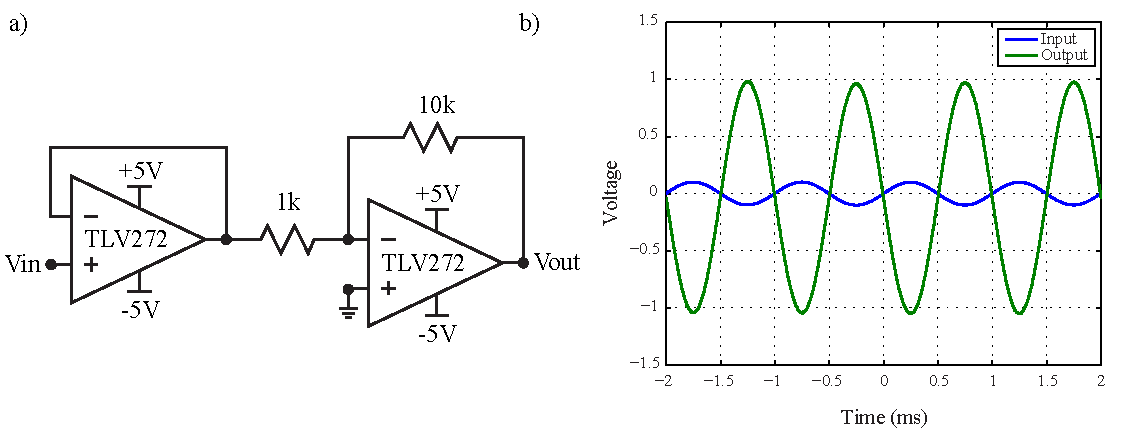
\includegraphics[width=1\textwidth]{Lab5demockt.pdf}
	\caption{Schematic for the demo circuit, a voltage follower followed by an inverting amplifier with a gain of 10 (a) and the resulting output (b)} \label{fig:5demockt}
\end{figure}

\begin{enumerate}
	\item Using only one of the TLV272 op amp in your lab parts kit, build the circuit in \hyperref[fig:5demockt]{Figure \ref*{fig:5demockt} (a)} on a breadboard. Set the voltage supplies to +/- 5 V and scope channel 1 to Vin and scope channel 2 to Vout. Configure the Wavegen to supply a 1 kHz sine wave with a 0.1 V amplitude. 
\end{enumerate}

%%%%%%%%%%%%%%%%%%%%%%%%%%%%%%%%%%%%%%%%%%%%%%%%%%%%%%%%%%%%%%%%%%%%%%%%%%%%%%%%%%%%%%%%%%%%%%%%%%%%%%%
\section{In-Lab Requirements}
%%%%%%%%%%%%%%%%%%%%%%%%%%%%%%%%%%%%%%%%%%%%%%%%%%%%%%%%%%%%%%%%%%%%%%%%%%%%%%%%%%%%%%%%%%%%%%%%%%%%%%%

The following must be completed at the start of lab. 

\begin{enumerate}
	\item All of the theoretical parameters from \hyperref[ssec:opampmodel]{Subsection \ref*{ssec:opampmodel}} tabled:
		\begin{enumerate}
			\item Offset voltage.
			\item Slew rate.
			\item Maximum output swing. 
			\item Effective gain. 
		\end{enumerate}
	\item Images of the output and circuits from \hyperref[ssec:opampmodel]{Subsection \ref*{ssec:opampmodel}} tabled:
		\begin{enumerate}
			\item \hyperref[itm:5ssec1itm5]{Item \ref*{itm:5ssec1itm5}}: Image of the circuit and the plot of the input and output voltage.
			\item \hyperref[itm:5ssec1itm6]{Item \ref*{itm:5ssec1itm6}}: Image of the circuit and the plot of the input and output voltage.
			\item \hyperref[itm:5ssec1itm7]{Item \ref*{itm:5ssec1itm7}}: Image of the circuit and the plot of effective gain.
		\end{enumerate}
	\item Op amp configurations from \hyperref[ssec:opampcon]{Subsection \ref*{ssec:opampcon}} built on a breadboard and working.
\end{enumerate}

%%%%%%%%%%%%%%%%%%%%%%%%%%%%%%%%%%%%%%%%%%%%%%%%%%%%%%%%%%%%%%%%%%%%%%%%%%%%%%%%%%%%%%%%%%%%%%%%%%%%%%%
\subsection{Experimental Op Amp Measurements}
%%%%%%%%%%%%%%%%%%%%%%%%%%%%%%%%%%%%%%%%%%%%%%%%%%%%%%%%%%%%%%%%%%%%%%%%%%%%%%%%%%%%%%%%%%%%%%%%%%%%%%%

Using the pre-built op amp configurations, complete the following.

\begin{enumerate}
	\item Using the voltage follower, \hyperref[fig:OAbuffer]{Figure \ref*{fig:OAbuffer}},input a 0 V DC voltage from the Wavgen and record the offset voltage. Choose an appropriate voltage scale, the voltage is on the order of mV. Save a screenshot of the waveform scope.
	\item Using the voltage follower again, \hyperref[fig:OAbuffer]{Figure \ref*{fig:OAbuffer}}, input a 0.5 V amplitude square wave with a 0.5 V offset from the Wavegen. Set the appropriate trigger and determine the slew rate in V/us. Save a screenshot of the waveform scope.
	\item Using the inverting amplifier, \hyperref[fig:OAconfigs]{Fiugre \ref*{fig:OAconfigs} (a)}, input a 1k Hz sine wave with a 1 V amplitude from the Wavegen. Determine the maximum output voltage swing. 
	\item Using the inverting amplifier again, \hyperref[fig:OAconfigs]{Fiugre \ref*{fig:OAconfigs} (a)}, input a 0.1 V DC from the Wavegen. Determine the effective gain. Choose an appropriate voltage scale for the input and output voltages. 
	\item Table all of values calculated in this subsection.
\end{enumerate}


%%%%%%%%%%%%%%%%%%%%%%%%%%%%%%%%%%%%%%%%%%%%%%%%%%%%%%%%%%%%%%%%%%%%%%%%%%%%%%%%%%%%%%%%%%%%%%%%%%%%%%%
\section{Write Up}
%%%%%%%%%%%%%%%%%%%%%%%%%%%%%%%%%%%%%%%%%%%%%%%%%%%%%%%%%%%%%%%%%%%%%%%%%%%%%%%%%%%%%%%%%%%%%%%%%%%%%%%

Include the following in the write up.

\begin{enumerate}
	\item Table of experimental parameters.
	\item Screenshots of scope output plots.
	\item Percent error, using the pre-lab values as the theoretical and the in-lab values as experimental.
\end{enumerate}

Discuss the differences between the ideal op amp model, spice TLV272 model, and the physical op amp focusing on the quantities calculated for this lab: offset voltage, slew rate, output voltage range, and effective gain. Touch on the following in your discussion.

\begin{itemize}
	\item When is it appropriate to use one model over the other?
	\item How accurate should the spice model for an op amp be?
\end{itemize}
For all lab write up submissions and reports the backgrounds for LTSpice and Waveforms should be changed from dark background to light background to make them readable for grading. 

If the prelab simulation is incorrect, do not compare the in lab results to wrong values.  Correct numbers or circuit schematics should be used in the write-up report.

\chapter{Lab 6 - Operational Amplifiers Applications}

%%%%%%%%%%%%%%%%%%%%%%%%%%%%%%%%%%%%%%%%%%%%%%%%%%%%%%%%%%%%%%%%%%%%%%%%%%%%%%%%%%%%%%%%%%%%%%%%%%%%%%%
\section{Objective}
%%%%%%%%%%%%%%%%%%%%%%%%%%%%%%%%%%%%%%%%%%%%%%%%%%%%%%%%%%%%%%%%%%%%%%%%%%%%%%%%%%%%%%%%%%%%%%%%%%%%%%%

The purpose of this lab is to delve in to the applications of operational amplifiers. There is an almost endless number of applications, the possibilities are often not intuitively obvious for students seeing them for the first time. 

%%%%%%%%%%%%%%%%%%%%%%%%%%%%%%%%%%%%%%%%%%%%%%%%%%%%%%%%%%%%%%%%%%%%%%%%%%%%%%%%%%%%%%%%%%%%%%%%%%%%%%%
\section{Materials}
%%%%%%%%%%%%%%%%%%%%%%%%%%%%%%%%%%%%%%%%%%%%%%%%%%%%%%%%%%%%%%%%%%%%%%%%%%%%%%%%%%%%%%%%%%%%%%%%%%%%%%%

\begin{itemize}
	\item Laptop with LTSpice
	\item Analog Discovery
	\item Breadboard
	\item Wiring kit
	\item Lab parts kit with TLV272 
\end{itemize}

%%%%%%%%%%%%%%%%%%%%%%%%%%%%%%%%%%%%%%%%%%%%%%%%%%%%%%%%%%%%%%%%%%%%%%%%%%%%%%%%%%%%%%%%%%%%%%%%%%%%%%%
\section{Introduction}
%%%%%%%%%%%%%%%%%%%%%%%%%%%%%%%%%%%%%%%%%%%%%%%%%%%%%%%%%%%%%%%%%%%%%%%%%%%%%%%%%%%%%%%%%%%%%%%%%%%%%%%

There are a variety of configurations op amps can be considered standard and while the simple inverting and non-inverting cases were show in Lab 5, here the pool is expanded to include a summing amplifier and a difference amplifier.

\begin{figure} [h!]
	\centering
		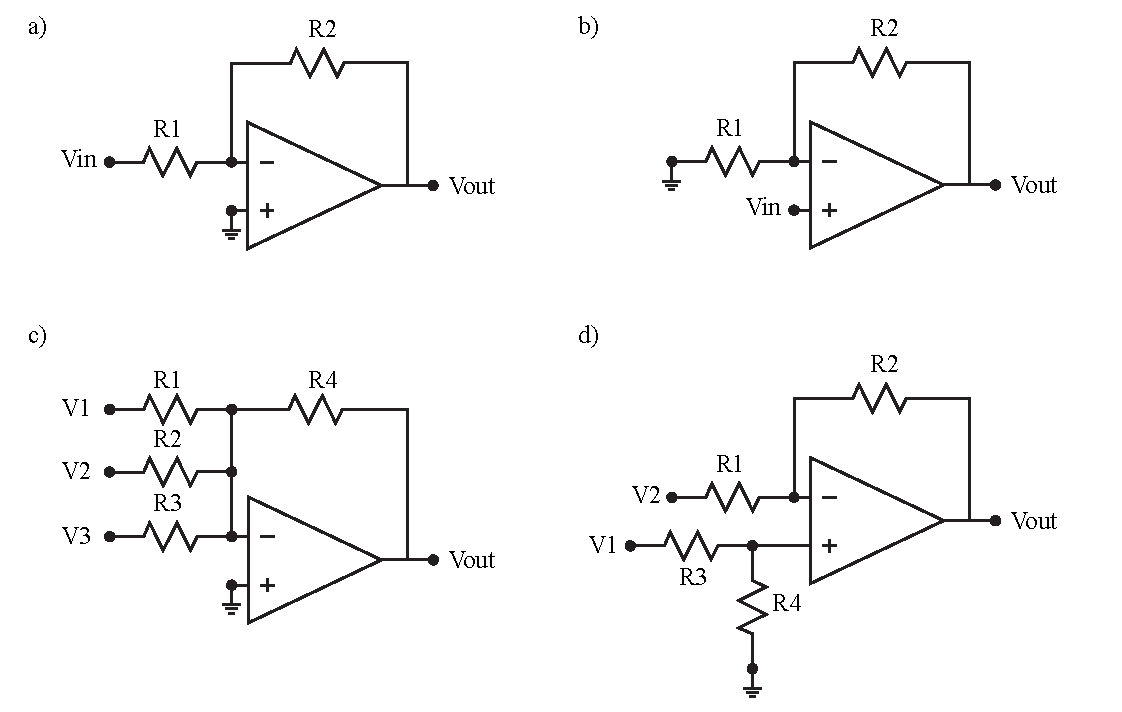
\includegraphics[width=1\textwidth]{Lab6configs.pdf}
	\caption{Different op amp configurations: inverting amplifier (a), non-inverting amplifier (b), summing amplifier (c), and difference amplifier (d).} \label{fig:6OAconfigs}
\end{figure}

%%%%%%%%%%%%%%%%%%%%%%%%%%%%%%%%%%%%%%%%%%%%%%%%%%%%%%%%%%%%%%%%%%%%%%%%%%%%%%%%%%%%%%%%%%%%%%%%%%%%%%
\subsubsection{Summing Amplifier}
%%%%%%%%%%%%%%%%%%%%%%%%%%%%%%%%%%%%%%%%%%%%%%%%%%%%%%%%%%%%%%%%%%%%%%%%%%%%%%%%%%%%%%%%%%%%%%%%%%%%%%

A summing amplifier, \hyperref[fig:6OAconfigs]{Figure \ref*{fig:6OAconfigs} (c)}, is effectively the same configuration as an inverting amplifier but has multiple inputs that allow for a weighted output voltage. 

\begin{equation}
	\centering
	V_{out} = -(\frac{R_4}{R_1}V_1 + \frac{R_4}{R_2}V_2 + \frac{R_4}{R_3}V_3)
\end{equation}

\noindent When the resistors $R_1$, $R_2$, $R_3$, and $R_4$ are all equal, the output voltage is an equal combination of the input voltages but the resistors can be chosen to weight the input voltages different based on the application. 


%%%%%%%%%%%%%%%%%%%%%%%%%%%%%%%%%%%%%%%%%%%%%%%%%%%%%%%%%%%%%%%%%%%%%%%%%%%%%%%%%%%%%%%%%%%%%%%%%%%%%%
\subsubsection{Difference Amplifier}
%%%%%%%%%%%%%%%%%%%%%%%%%%%%%%%%%%%%%%%%%%%%%%%%%%%%%%%%%%%%%%%%%%%%%%%%%%%%%%%%%%%%%%%%%%%%%%%%%%%%%%

Difference amplifiers, \hyperref[fig:6OAconfigs]{Figure \ref*{fig:6OAconfigs} (d)}, as the name implies takes the difference between the two input voltages resulting in that depends on the ratios of resistor values.

\begin{equation}
	\centering
	V_{out} =  V_1 \left(\frac{R_2}{R_1+R_2}\right)\left(\frac{R_3+R_4}{R_3}\right)-V_2\frac{R_4}{R_3}  
\end{equation}

\noindent When the resistors $R_1 = R_3$ and $R_2 = R_4$ the output voltage simplifies to 

\begin{equation}
	\centering
	V_{out} =  (V_1-V_2)\frac{R_2}{R_1}  
\end{equation}

%%%%%%%%%%%%%%%%%%%%%%%%%%%%%%%%%%%%%%%%%%%%%%%%%%%%%%%%%%%%%%%%%%%%%%%%%%%%%%%%%%%%%%%%%%%%%%%%%%%%%%%
\section{Big Picture}
%%%%%%%%%%%%%%%%%%%%%%%%%%%%%%%%%%%%%%%%%%%%%%%%%%%%%%%%%%%%%%%%%%%%%%%%%%%%%%%%%%%%%%%%%%%%%%%%%%%%%%%

\begin{figure} [h]
	\centering
		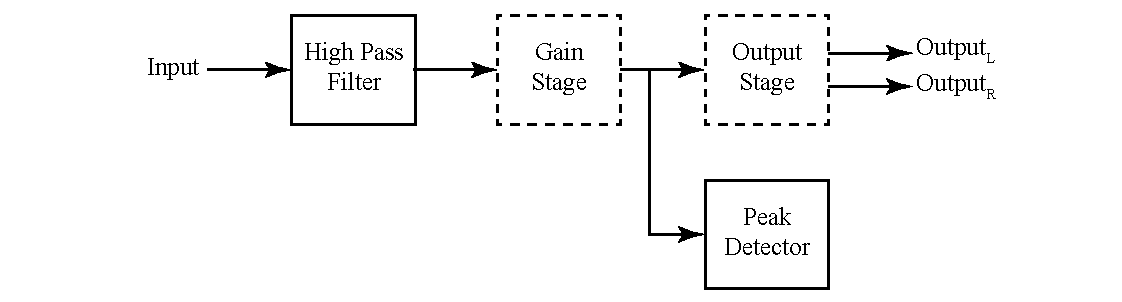
\includegraphics[width=1\textwidth]{Lab5bigpicture.pdf}
	\caption{Big picture with emphasis on the gain and output stages.} \label{fig:6bp}
\end{figure}

This lab again focuses on op amps but op amps used as different building blocks to compose more complicated circuits. The final project circuit is about as complicated as the final circuit in this lab. 

%%%%%%%%%%%%%%%%%%%%%%%%%%%%%%%%%%%%%%%%%%%%%%%%%%%%%%%%%%%%%%%%%%%%%%%%%%%%%%%%%%%%%%%%%%%%%%%%%%%%%%%
\section{Pre-Lab Requirements}
%%%%%%%%%%%%%%%%%%%%%%%%%%%%%%%%%%%%%%%%%%%%%%%%%%%%%%%%%%%%%%%%%%%%%%%%%%%%%%%%%%%%%%%%%%%%%%%%%%%%%%%

Complete the following before coming to lab. 

%%%%%%%%%%%%%%%%%%%%%%%%%%%%%%%%%%%%%%%%%%%%%%%%%%%%%%%%%%%%%%%%%%%%%%%%%%%%%%%%%%%%%%%%%%%%%%%%%%%%%%%
\subsection{Buffering} \label{ssec:6buff}
%%%%%%%%%%%%%%%%%%%%%%%%%%%%%%%%%%%%%%%%%%%%%%%%%%%%%%%%%%%%%%%%%%%%%%%%%%%%%%%%%%%%%%%%%%%%%%%%%%%%%%%

Buffering is an important op amp application because it solves a problem, loading effects, that can't easily be solved with purely resistive circuits. 

\begin{figure} [h]
	\centering
		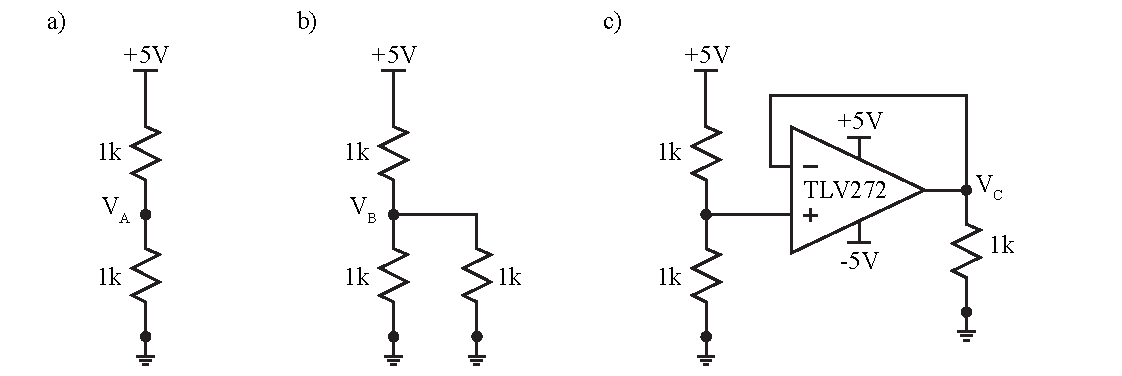
\includegraphics[width=1\textwidth]{Lab6buffering.pdf}
	\caption{A simple voltage divider (a), voltage divider with a load (b), and a voltage divider with a voltage follower between the output and the load (c).} \label{fig:6buff}
\end{figure}

\begin{enumerate}
	\item Simulate  all three circuits in \hyperref[fig:6buff]{Figure \ref*{fig:6buff}} using a DC operating point (.op). Keep all the circuits on the same schematic and table the voltages $V_A$, $V_B$, and $V_C$. Save an image of the circuit and submit the image and table in a document to Canvas. \label{itm:6ssec1itm1}
	\item Discuss why two of the voltages are approximately 2.5 V but one is not. Submit your answer as part of the document submitted to Canvas. \label{itm:6ssec1itm2}
\end{enumerate}

%%%%%%%%%%%%%%%%%%%%%%%%%%%%%%%%%%%%%%%%%%%%%%%%%%%%%%%%%%%%%%%%%%%%%%%%%%%%%%%%%%%%%%%%%%%%%%%%%%%%%%%
\subsection{Level Shifting} \label{ssec:6lvlshift}
%%%%%%%%%%%%%%%%%%%%%%%%%%%%%%%%%%%%%%%%%%%%%%%%%%%%%%%%%%%%%%%%%%%%%%%%%%%%%%%%%%%%%%%%%%%%%%%%%%%%%%%

Level shifting in electronic circuits is the process of change the supply rails from one range to another. For example, when preparing a signal for analog to digital conversion, the signal may be bi-polar (+/-) and must be converted to a single voltage rail. So, instead of a sine wave that swings to +2.5V and -2.5V, 2.5V is added so that the sine wave swings from +5V to 0V with the same amplitude. 

\begin{figure} [h]
	\centering
		\includegraphics[width=1\textwidth]{Lab6levelshift.pdf}
	\caption{A summing amplifier used to add 2.5V to $-V_{IN}$ (a) and the same configuration where the -2.5V source has been replaced with a buffered voltage divider (b).} \label{fig:6levelshift}
\end{figure}

\begin{enumerate}
	\item Simulate the circuit in \hyperref[fig:6levelshift]{Figure \ref*{fig:6levelshift} (a)} using a transient analysis with a stop time of 1m (.tran 1m). Set $V_{S}$ to a sine wave with a 0 V DC offset, 2 V amplitude, and a 1 kHz frequency. Save an image of the circuit and a plot of the input and output voltage for submission to Canvas. \label{itm:6ssec2itm1}
	\item Explain why the resistor divider in \hyperref[fig:6levelshift]{Figure \ref*{fig:6levelshift} (b)} uses -5V instead of 5V. Submit your answer as part of the document submitted to Canvas. \label{itm:6ssec2itm2}
	\item Practically, a 2.5V reference may not be available for use and instead must be self generated. Simulate the circuit in \hyperref[fig:6levelshift]{Figure \ref*{fig:6levelshift} (b)} using a transient analysis with a stop time of 1m (.tran 1m). Set $V_{S}$ to a sine wave with a 0 V DC offset, 2 V amplitude, and a 1 kHz frequency. Save an image of the circuit and a plot of the input and output voltage for submission to Canvas. \label{itm:6ssec2itm3}
	\item Construct the circuit in \hyperref[fig:6levelshift]{Figure \ref*{fig:6levelshift} (b)} on a breadboard. Configure the Wavegen to generate a sine wave at 1 kHz with a 2 amplitude and a 0V offset. Plot the input and output on the Scope and save the circuit to demo at the start of lab. \label{itm:6ssec2itm4}
	\item In the more general case, the full range of input must be accounted for. Simulate the circuit in \hyperref[fig:6fullshift]{Figure \ref*{fig:6fullshift}} using a transient analysis with a stop time of 1m (.tran 1m). Set $V_{IN}$ to a sine wave with a 0 V DC offset, 5 V amplitude, and a 1 kHz frequency. Save an image of the circuit and a plot of the input and output voltage for submission to Canvas. \label{itm:6ssec2itm5}
\end{enumerate}

\begin{figure} [h]
	\centering
		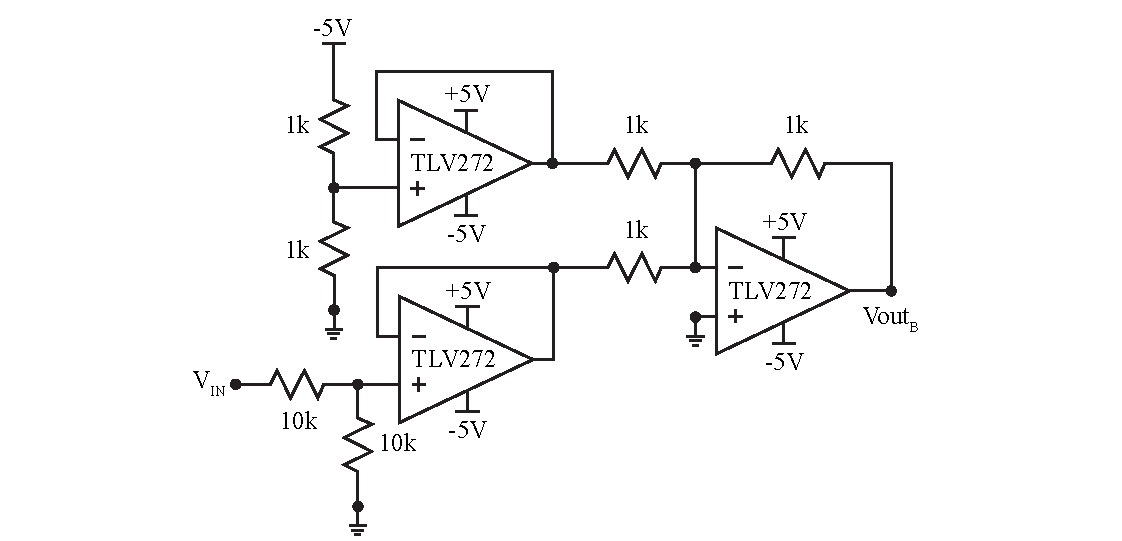
\includegraphics[width=1\textwidth]{Lab6fullshift.pdf}
	\caption{A DC level shifter configured to convert the full range of +/-5 to +5/0.} \label{fig:6fullshift}
\end{figure}

\newpage

%%%%%%%%%%%%%%%%%%%%%%%%%%%%%%%%%%%%%%%%%%%%%%%%%%%%%%%%%%%%%%%%%%%%%%%%%%%%%%%%%%%%%%%%%%%%%%%%%%%%%%%
\subsection{Differential to Single Ended Conversion} \label{ssec:6diff2single}
%%%%%%%%%%%%%%%%%%%%%%%%%%%%%%%%%%%%%%%%%%%%%%%%%%%%%%%%%%%%%%%%%%%%%%%%%%%%%%%%%%%%%%%%%%%%%%%%%%%%%%%

Differential signals, two signals where one signal is 180 degrees out of phase with the other signal, have a variety of applications. The primary benefit of differential signals is increased noise performance but at the cost of extra hardware, you need two of everything. Converting from a differential signal to a singled ended signal can be accomplished fairly simply with a difference amplifier. 

\begin{figure} [h]
	\centering
		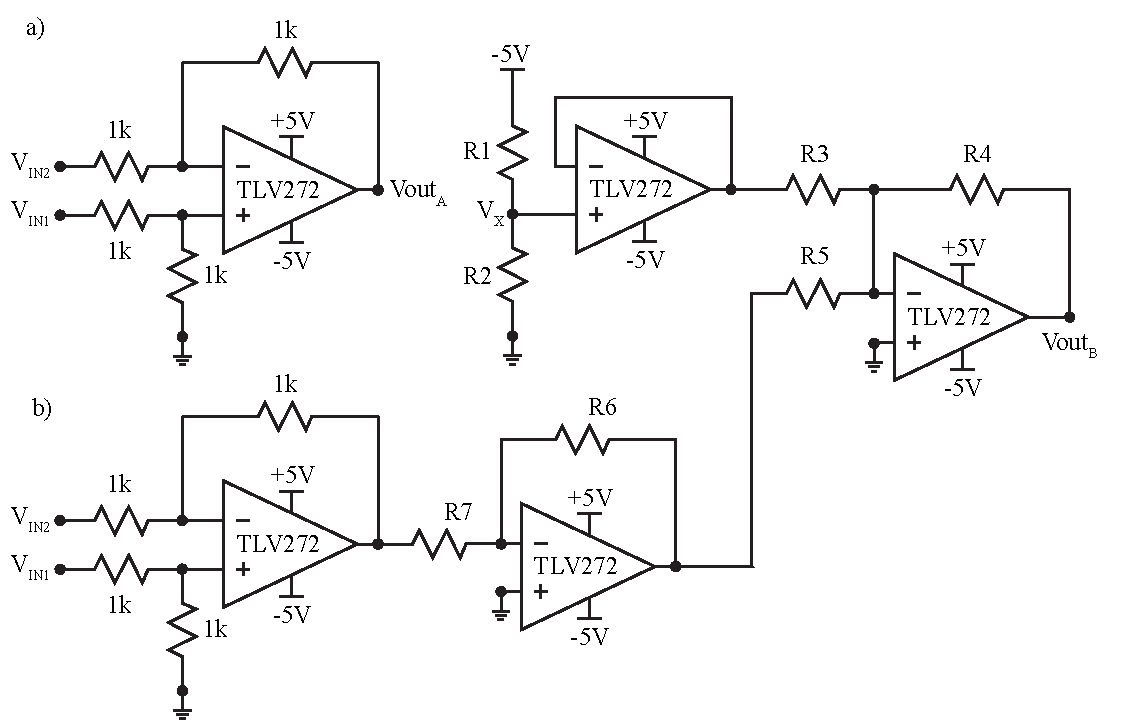
\includegraphics[width=1\textwidth]{Lab6difftosingle.pdf}
	\caption{A difference amplifier that converts a differential signal to single ended (a) and a combination of the level shifter and differential to single ended converter (b).} \label{fig:6difftosingle}
\end{figure}

\begin{enumerate}
	\item Simulate the circuit in \hyperref[fig:6difftosingle]{Figure \ref*{fig:6difftosingle} (a)} using a transient analysis with a stop time of 1m (.tran 1m). Set $V_{IN1}$ to a sine wave with a 0 V DC offset, 0.5 V amplitude, and a 1k Hz frequency. Set $V_{IN2}$ to a sine wave with a 0 V DC offset, 0.5 V amplitude, a 1k Hz frequency, and a phase of 180 degrees. Save an image of the circuit and a plot of the input (both inputs) and output voltages for submission to Canvas. \label{itm:6ssec3itm1}
	\item Determine the resistor values for R1 through R7, recall that there are limited quantities in the lab kit. Choose R1 and R2 so that $V_X$ is 2.5V, R3, R4, and R5 so that both voltages are added equally, and R6 and R7 so that the output, $Vout_B$ utilizes as much of the full range, 0 to 5V, as possible without clipping. \label{itm:6ssec3itm2}
	\item Simulate the circuit in \hyperref[fig:6difftosingle]{Figure \ref*{fig:6difftosingle} (b)} using a transient analysis with a stop time of 1m (.tran 1m). Set $V_{S1}$ and $V_{S2}$ to their previously defined values. Save an image of the circuit and a plot of the input (both inputs) and output voltages for submission to Canvas. \label{itm:6ssec3itm3}
	\item Explain how the circuit in \hyperref[fig:6difftosingle]{Figure \ref*{fig:6difftosingle} (b)} works  in a few sentences. Submit your answer as part of the document submitted to Canvas. \label{itm:6ssec3itm4}
\end{enumerate}

\newpage

%%%%%%%%%%%%%%%%%%%%%%%%%%%%%%%%%%%%%%%%%%%%%%%%%%%%%%%%%%%%%%%%%%%%%%%%%%%%%%%%%%%%%%%%%%%%%%%%%%%%%%%
\section{In-Lab Requirements}
%%%%%%%%%%%%%%%%%%%%%%%%%%%%%%%%%%%%%%%%%%%%%%%%%%%%%%%%%%%%%%%%%%%%%%%%%%%%%%%%%%%%%%%%%%%%%%%%%%%%%%%

The following must be completed at the start of lab. 

\begin{enumerate}
	\item \hyperref[ssec:6buff]{Section \ref*{ssec:6buff}}
		\begin{enumerate}
			\item \hyperref[itm:6ssec1itm1]{Item \ref*{itm:6ssec1itm1}}: Image of the circuit and a table of output voltages.
			\item \hyperref[itm:6ssec1itm2]{Item \ref*{itm:6ssec1itm2}}: Answer to question.
		\end{enumerate}
	\item \hyperref[ssec:6lvlshift]{Section \ref*{ssec:6lvlshift}}
		\begin{enumerate}
			\item \hyperref[itm:6ssec2itm1]{Item \ref*{itm:6ssec2itm1}}: Image of the circuit and a plot of the input and output voltages.
			\item \hyperref[itm:6ssec2itm2]{Item \ref*{itm:6ssec2itm2}}: Answer to question.
			\item \hyperref[itm:6ssec2itm3]{Item \ref*{itm:6ssec2itm3}}: Image of the circuit and a plot of the input and output voltages.
			\item \hyperref[itm:6ssec2itm4]{Item \ref*{itm:6ssec2itm4}}: Plot of the input and output voltages and a circuit demonstration.
			\item \hyperref[itm:6ssec2itm4]{Item \ref*{itm:6ssec2itm5}}: Image of the circuit and a plot of the input and output voltages.
		\end{enumerate}
	\item \hyperref[ssec:6diff2single]{Section \ref*{ssec:6diff2single}}
		\begin{enumerate}
			\item \hyperref[itm:6ssec3itm1]{Item \ref*{itm:6ssec3itm1}}: Image of the circuit and a plot of the input and output voltages.
			\item \hyperref[itm:6ssec3itm3]{Item \ref*{itm:6ssec3itm3}}: Image of the circuit and a plot of the input and output voltages.
			\item \hyperref[itm:6ssec3itm4]{Item \ref*{itm:6ssec3itm4}}: Answer to question.
		\end{enumerate}
\end{enumerate}

Complete the following in lab.

%%%%%%%%%%%%%%%%%%%%%%%%%%%%%%%%%%%%%%%%%%%%%%%%%%%%%%%%%%%%%%%%%%%%%%%%%%%%%%%%%%%%%%%%%%%%%%%%%%%%%%%
\subsection{Construction} \label{ssec:6const}
%%%%%%%%%%%%%%%%%%%%%%%%%%%%%%%%%%%%%%%%%%%%%%%%%%%%%%%%%%%%%%%%%%%%%%%%%%%%%%%%%%%%%%%%%%%%%%%%%%%%%%%

\begin{enumerate}
	\item Construct the circuit from \hyperref[itm:6ssec2itm5]{Section \ref*{ssec:6lvlshift} Item \ref*{itm:6ssec2itm5}}. Set Wavegen1, $V_{IN}$, to a sine wave with a 5 V amplitude, 0 V offset, and a frequency of 1 kHz. \label{itm:6ssec4itm1}
	\item Plot the input and output voltages, save an image of the plot. \label{itm:6ssec4itm2}
	\item Construct the circuit from \hyperref[itm:6ssec3itm3]{Section \ref*{ssec:6diff2single} Item \ref*{itm:6ssec3itm3}}. Set Wavegen1 to $V_{IN1}$ and Wavegen2 to $V_{IN2}$. \label{itm:6ssec4itm3} Synchronize wavegen1 and wavegen2 using the dropdown in the wavegen tab of waveforms. It is located two tabs to the right of "Run all" and is defaulted to "No synchronization".
	\item Plot the input (differential) and the output voltages, save an image of the plot. \label{itm:6ssec4itm4}
\end{enumerate}



%%%%%%%%%%%%%%%%%%%%%%%%%%%%%%%%%%%%%%%%%%%%%%%%%%%%%%%%%%%%%%%%%%%%%%%%%%%%%%%%%%%%%%%%%%%%%%%%%%%%%%%
\section{Write Up}
%%%%%%%%%%%%%%%%%%%%%%%%%%%%%%%%%%%%%%%%%%%%%%%%%%%%%%%%%%%%%%%%%%%%%%%%%%%%%%%%%%%%%%%%%%%%%%%%%%%%%%%

Include the following in the write up.

\begin{enumerate}
	\item \hyperref[ssec:6const]{Section \ref*{ssec:6const}}
		\begin{enumerate}
			\item \hyperref[itm:6ssec4itm1]{Item \ref*{itm:6ssec4itm1}}: Schematic of the circuit, do not copy the schematic from the lab manual, an image from LTspice is fine. 
			\item \hyperref[itm:6ssec4itm2]{Item \ref*{itm:6ssec4itm2}}: Plot of the input and output voltages. 
			\item \hyperref[itm:6ssec4itm1]{Item \ref*{itm:6ssec4itm3}}: Schematic of the circuit, do not copy the schematic from the lab manual, an image from LTspice is fine. 
			\item \hyperref[itm:6ssec4itm2]{Item \ref*{itm:6ssec4itm4}}: Plot of the input and output voltages. 
		\end{enumerate}
\end{enumerate}

Discuss the two circuits constructed in lab. Explain how each circuit works at the block level and how resistor tolerance could or could not have an effect on the output. Also explain the design choices for the circuit, \hyperref[itm:6ssec3itm3]{Section \ref*{ssec:6diff2single} Item \ref*{itm:6ssec3itm3}}, constructed in lab. Which resistors were chosen and why? 

\chapter{Lab 7 - Capacitor Applications}

%%%%%%%%%%%%%%%%%%%%%%%%%%%%%%%%%%%%%%%%%%%%%%%%%%%%%%%%%%%%%%%%%%%%%%%%%%%%%%%%%%%%%%%%%%%%%%%%%%%%%%%
\section{Objective}
%%%%%%%%%%%%%%%%%%%%%%%%%%%%%%%%%%%%%%%%%%%%%%%%%%%%%%%%%%%%%%%%%%%%%%%%%%%%%%%%%%%%%%%%%%%%%%%%%%%%%%%

The objective of this lab is to introduce another fundamental circuit element, the capacitor, and their applications within certain circuits. Specifiably for this lab, the focus is on a capacitor used in conjunction with a 555 timer. 

%%%%%%%%%%%%%%%%%%%%%%%%%%%%%%%%%%%%%%%%%%%%%%%%%%%%%%%%%%%%%%%%%%%%%%%%%%%%%%%%%%%%%%%%%%%%%%%%%%%%%%%
\section{Materials}
%%%%%%%%%%%%%%%%%%%%%%%%%%%%%%%%%%%%%%%%%%%%%%%%%%%%%%%%%%%%%%%%%%%%%%%%%%%%%%%%%%%%%%%%%%%%%%%%%%%%%%%

\begin{itemize}
	\item Laptop with LTSpice
	\item Analog Discovery
	\item Breadboard
	\item Wiring kit
	\item Lab parts kit 
\end{itemize}

%%%%%%%%%%%%%%%%%%%%%%%%%%%%%%%%%%%%%%%%%%%%%%%%%%%%%%%%%%%%%%%%%%%%%%%%%%%%%%%%%%%%%%%%%%%%%%%%%%%%%%%
\section{Introduction}
%%%%%%%%%%%%%%%%%%%%%%%%%%%%%%%%%%%%%%%%%%%%%%%%%%%%%%%%%%%%%%%%%%%%%%%%%%%%%%%%%%%%%%%%%%%%%%%%%%%%%%%

There are a variety of applications of capacitors which could fill an entire class. The focus for this lab will be the use of a capacitor and its associated RC time constant in conjunction with a 555 timer. 

%%%%%%%%%%%%%%%%%%%%%%%%%%%%%%%%%%%%%%%%%%%%%%%%%%%%%%%%%%%%%%%%%%%%%%%%%%%%%%%%%%%%%%%%%%%%%%%%%%%%%%%
\subsection{Time Domain Response}
%%%%%%%%%%%%%%%%%%%%%%%%%%%%%%%%%%%%%%%%%%%%%%%%%%%%%%%%%%%%%%%%%%%%%%%%%%%%%%%%%%%%%%%%%%%%%%%%%%%%%%%

While the operation of a capacitor can be analyzed in both the time and frequency domains, the focus here is on the time domain. 

\begin{figure}
	\centering
		\includegraphics[width=1\textwidth]{Lab5cap.pdf}
	\caption{A simple RC circuit (a) and the associated input and output (b). Note that the input is the node after the switch in (a).} \label{fig:capoutput}
\end{figure}

A simple RC circuit with a switch as shown in \hyperref[fig:capoutput]{Figure \ref*{fig:capoutput}} will charge and discharge as the 1 V source is connected and disconnected. Charging to the source voltage takes the form of 

\begin{equation}
	\centering
	V_{out} = 1 - V_{in}e^{-t/\tau}
\end{equation}

\noindent where $\tau = RC$ and discharging takes the form

\begin{equation}
	\centering
	V_{out} =  V_{in}e^{-t/\tau}
\end{equation}

\noindent While the result is novel and opens up a lot of possibilities, there isn't a clear path to the actual application of the capacitor. Sure, it can be used in the previously mentioned simple RC circuit, but there isn't a clear use. Enter the 555 timer, an early chip that because incredibly popular due to the ability to generate various timing signals using external components to set an RC time constant. 

%%%%%%%%%%%%%%%%%%%%%%%%%%%%%%%%%%%%%%%%%%%%%%%%%%%%%%%%%%%%%%%%%%%%%%%%%%%%%%%%%%%%%%%%%%%%%%%%%%%%%%%
\subsection{555 Timer}
%%%%%%%%%%%%%%%%%%%%%%%%%%%%%%%%%%%%%%%%%%%%%%%%%%%%%%%%%%%%%%%%%%%%%%%%%%%%%%%%%%%%%%%%%%%%%%%%%%%%%%%

A 555 timer can operate in two modes, mono-stable  and a-stable. Mono-stable operating is when the circuit will only output once when triggered and will wait for future triggers to output again. A-stable operating requires no input and will internally trigger to perpetually produce output. 

For clarification, there is a distinction between the pulse duration, the time a signal is high (highest positive voltage, usually the positive voltage rail) and the period. \hyperref[fig:7durvsper]{Figure \ref*{fig:7durvsper}} shows the difference between the pulse duration and period for a square wave. The pulse duration is time the square wave is at its maximum value, 1 V in this case, for a total of 0.25 ms. While the period is the time it takes for the signal to repeat, 0.5 ms. 

\begin{figure}
	\centering
		\includegraphics[width=0.5\textwidth]{lab7durvsper.pdf}
	\caption{A plot of a square wave with the pulse duration and period labeled.} \label{fig:7durvsper}
\end{figure}

\newpage

%%%%%%%%%%%%%%%%%%%%%%%%%%%%%%%%%%%%%%%%%%%%%%%%%%%%%%%%%%%%%%%%%%%%%%%%%%%%%%%%%%%%%%%%%%%%%%%%%%%%%%%
\subsubsection{Mono-Stable Configuration}
%%%%%%%%%%%%%%%%%%%%%%%%%%%%%%%%%%%%%%%%%%%%%%%%%%%%%%%%%%%%%%%%%%%%%%%%%%%%%%%%%%%%%%%%%%%%%%%%%%%%%%%

The mono-stable configuration, \hyperref[fig:monostable]{Figure \ref*{fig:monostable}}, requires an input and only triggers when that input passes below a specific threshold (active low). Once the input falls below the threshold voltage, the output goes to 5 V for $t=  1.1 R_A C_L$ and the capacitor starts to charge. Once the capacitor voltage reaches a threshold, the output and the capacitor voltage both go to zero and the circuit waits for the input voltage to go zero again. 

\begin{figure}
	\centering
		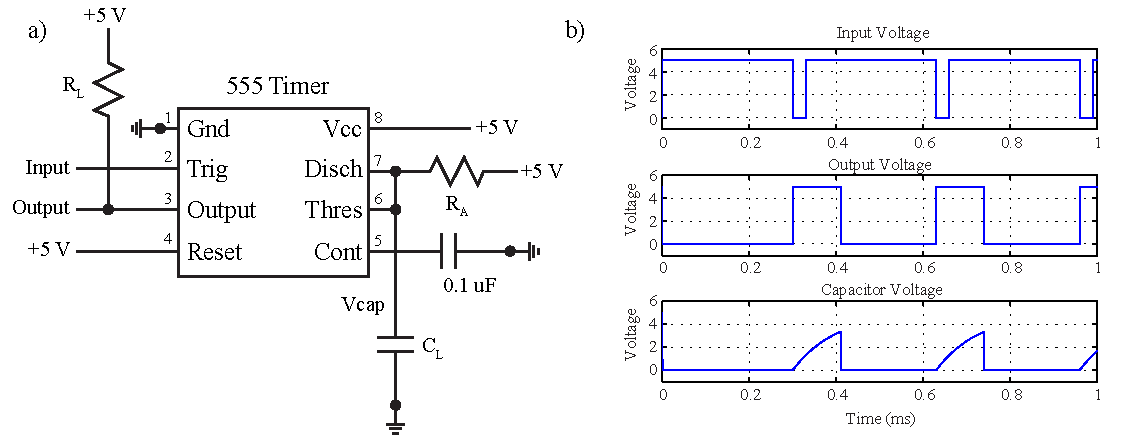
\includegraphics[width=0.9\textwidth]{Lab5monostable.pdf}
	\caption{The circuit for mono-stable operation (a) and the output voltages (b). Vcc is 5 V, $R_L = 1\mathrm{k}\; \Omega$, $C_L = 0.01\mu \mathrm{F}$, and $R_A = 10\mathrm{k}\;\Omega$. Note that wires that cross are only connected if there is a dot at the junction.} \label{fig:monostable}
\end{figure}



%%%%%%%%%%%%%%%%%%%%%%%%%%%%%%%%%%%%%%%%%%%%%%%%%%%%%%%%%%%%%%%%%%%%%%%%%%%%%%%%%%%%%%%%%%%%%%%%%%%%%%%
\subsubsection{A-Stable Configuration}
%%%%%%%%%%%%%%%%%%%%%%%%%%%%%%%%%%%%%%%%%%%%%%%%%%%%%%%%%%%%%%%%%%%%%%%%%%%%%%%%%%%%%%%%%%%%%%%%%%%%%%%

The a-stable configuration, \hyperref[fig:astable]{Figure \ref*{fig:astable}}, does not require an input  and utilizes the charging and discharging of the capacitor to trigger the input. With the addition of a second resistor, $R_B$, the capacitor will charge through resistors $R_A$ and $R_B$ but the capacitor will only discharge through $R_B$, leading to two different time constants. 

As the capacitor discharges, the output is zero until the capacitor voltage reaches the lower threshold voltages and then the output goes to 5 V until the capacitor voltage reaches the upper threshold and the process repeats. 

\begin{figure}[h]
	\centering
		\includegraphics[width=0.9\textwidth]{Lab5astable.pdf}
	\caption{The circuit for a-stable operation (a) and the output voltages (b). Vcc is 5 V, $R_L = 1\mathrm{k}\; \Omega$, $C_L = 0.01\mu \mathrm{F}$, $R_A = 10k\;\Omega$, and $R_B = 10\mathrm{k}\;\Omega$. Note that wires that cross are only connected if there is a dot at the junction.} \label{fig:astable}
\end{figure}

The time that the output is high is set by the two resistors and capacitor:

\begin{equation}
	\centering
	t_H = 0.693(R_A + R_B)C_L
\end{equation}

\noindent While the time the output is low is only set by $R_B$ and the capacitor:

\begin{equation}
	\centering
	t_L = 0.693(R_B)C_L
\end{equation}

%%%%%%%%%%%%%%%%%%%%%%%%%%%%%%%%%%%%%%%%%%%%%%%%%%%%%%%%%%%%%%%%%%%%%%%%%%%%%%%%%%%%%%%%%%%%%%%%%%%%%%%
\section{Big Picture}
%%%%%%%%%%%%%%%%%%%%%%%%%%%%%%%%%%%%%%%%%%%%%%%%%%%%%%%%%%%%%%%%%%%%%%%%%%%%%%%%%%%%%%%%%%%%%%%%%%%%%%%

While capacitors are used in the finale project, they're used for filtering purposes as opposed to use in the time domain with the 555 timer. 

%%%%%%%%%%%%%%%%%%%%%%%%%%%%%%%%%%%%%%%%%%%%%%%%%%%%%%%%%%%%%%%%%%%%%%%%%%%%%%%%%%%%%%%%%%%%%%%%%%%%%%%
\section{Pre-Lab Requirements}
%%%%%%%%%%%%%%%%%%%%%%%%%%%%%%%%%%%%%%%%%%%%%%%%%%%%%%%%%%%%%%%%%%%%%%%%%%%%%%%%%%%%%%%%%%%%%%%%%%%%%%%

Complete the following before coming to lab. 

%%%%%%%%%%%%%%%%%%%%%%%%%%%%%%%%%%%%%%%%%%%%%%%%%%%%%%%%%%%%%%%%%%%%%%%%%%%%%%%%%%%%%%%%%%%%%%%%%%%%%%%
\subsection{LTspice Simulations} \label{ssec:sims}
%%%%%%%%%%%%%%%%%%%%%%%%%%%%%%%%%%%%%%%%%%%%%%%%%%%%%%%%%%%%%%%%%%%%%%%%%%%%%%%%%%%%%%%%%%%%%%%%%%%%%%%

Using LTspice, complete the following. Use 5 V for Vcc, $R_L = 1\mathrm{k}\;\Omega$, and the NE555 model for the 555 timer found in the Misc component section. 

\begin{enumerate}
	\item Read the NE555 datasheet, \url{http://www.ti.com/product/NE555/datasheet}. Please note that a mono-stable allows for the pulse width to change as resistor and capacitor values are varied, while an a-stable configuration allows for the period the be varied as resistor and capacitor values are varied.
	\item Using the mono-stable configuration, determine the output when $R_A = 15\mathrm{k}\;\Omega$ and $C_L = 0.01 \mu \mathrm{F}$. Set the input to a pulse source with the following settings: 0 5 0 1n 1n 0.2m 0.25m 5 and run a transient simulation with a stop time of 1m (.tran 1m). Table the output voltage pulse duration, then save an image of the circuit and a plot of the input and output voltage for submission to Canvas. \label{itm:7ssec1itm1}
	\item Using the mono-stable configuration, choose $R_A$ and $C_L$ so that the output pulse duration is  approximtely 200 $\mu$s ($f\approx 5$ kHz) for a 100 kHz input; the solution should be withing 4 $\mu$s, 200 $\mu$s +/- 4 $\mu$s (5 kHz +/- 100 Hz). Use only the parts in your lab kit. Set the input to a pulse source with the following settings: 0 5 0 1n 1n 8u 10u 50 and run a transient simulation with a stop time of 0.5m (.tran 0.5m). Table the output voltage pulse duration, then save an image of the circuit and a plot of the input and output voltage for submission to Canvas. \label{itm:7ssec1itm2}
	\item Using the a-stable configuration, determine the output when $R_A = 10\mathrm{k}\;\Omega$, $R_B = 10\mathrm{k}\;\Omega$, and $C_L = 0.01 \mu \mathrm{F}$. Run a transient simulation with a stop time of 1m (.tran 1m). Table the output voltage period, then save an image of the circuit and a plot of the output voltage for submission to Canvas. \label{itm:7ssec1itm3}
	\item Using the a-stable configuration, choose $R_A$, $R_B$, and $C_L$ so that the frequency of the output signal is 10 kHz, there is an exact solution. Use only the parts in your lab kit. Run a transient simulation with a stop time of 0.5m (.tran 0.5m). Table the output voltage period, then save an image of the circuit and a plot of the output voltage for submission to Canvas. \label{itm:7ssec1itm4}
\end{enumerate}

%%%%%%%%%%%%%%%%%%%%%%%%%%%%%%%%%%%%%%%%%%%%%%%%%%%%%%%%%%%%%%%%%%%%%%%%%%%%%%%%%%%%%%%%%%%%%%%%%%%%%%%
\subsection{Breadboard Implementation} \label{ssec:breadboard}
%%%%%%%%%%%%%%%%%%%%%%%%%%%%%%%%%%%%%%%%%%%%%%%%%%%%%%%%%%%%%%%%%%%%%%%%%%%%%%%%%%%%%%%%%%%%%%%%%%%%%%%

\begin{enumerate}
	\item Build a mono-stable configuration  from \hyperref[itm:7ssec1itm1]{Section \ref*{ssec:sims} Item \ref*{itm:7ssec1itm1}}. Set Vcc to 5 V supply and use a 5 kHz square wave as the input with a 2.5 V amplitude and a 2.5 V offset. You can determine the capacitor values by their quantity or the labels: 102J - 0.001 $\mu$F, 103J - 0.01 $\mu$F, 333J - 0.033 $\mu$F, 473J - 0.047 $\mu$ F, 104J - 0.1 $\mu$ F, and 105K - 1 $\mu$F.
	\item Display the output voltage and the capacitor voltage on the o-scope to demonstrate the circuit to your lab instructor at the start of lab. In this case it helps to ground the negative terminals for the o-scope probes. 
\end{enumerate}

%%%%%%%%%%%%%%%%%%%%%%%%%%%%%%%%%%%%%%%%%%%%%%%%%%%%%%%%%%%%%%%%%%%%%%%%%%%%%%%%%%%%%%%%%%%%%%%%%%%%%%%
\section{In-Lab Requirements}
%%%%%%%%%%%%%%%%%%%%%%%%%%%%%%%%%%%%%%%%%%%%%%%%%%%%%%%%%%%%%%%%%%%%%%%%%%%%%%%%%%%%%%%%%%%%%%%%%%%%%%%

The following must be completed at the start of lab. 

\begin{enumerate}
	\item \hyperref[ssec:sims]{Subsection \ref*{ssec:sims}}
		\begin{enumerate} 
			\item \hyperref[itm:7ssec1itm1]{Item \ref*{itm:7ssec1itm1}}: An image of the circuit and a plot of the input and output voltage.
			\item \hyperref[itm:7ssec1itm2]{Item \ref*{itm:7ssec1itm2}}: An image of the circuit and a plot of the input and output voltage.
			\item \hyperref[itm:7ssec1itm3]{Item \ref*{itm:7ssec1itm3}}: An image of the circuit and a plot of the output voltage.
			\item \hyperref[itm:7ssec1itm4]{Item \ref*{itm:7ssec1itm4}}: An image of the circuit and a plot of the output voltage.
			\item Table of both theoretical pulse durations and periods. 
		\end{enumerate}
		\begin{enumerate}
			\item \hyperref[ssec:breadboard]{Section \ref*{ssec:breadboard}}: Mono-stable configuration implemented and working on a breadboard. 
		\end{enumerate}

\end{enumerate}

%%%%%%%%%%%%%%%%%%%%%%%%%%%%%%%%%%%%%%%%%%%%%%%%%%%%%%%%%%%%%%%%%%%%%%%%%%%%%%%%%%%%%%%%%%%%%%%%%%%%%%%
\subsection{Construction}
%%%%%%%%%%%%%%%%%%%%%%%%%%%%%%%%%%%%%%%%%%%%%%%%%%%%%%%%%%%%%%%%%%%%%%%%%%%%%%%%%%%%%%%%%%%%%%%%%%%%%%%

For all four cases, determine the experimental pulse durations/periods for the output voltage and table the resulting values. 

\begin{enumerate}
	\item Save an image of the output voltage and capacitor voltage on the o-scope for the circuit from \hyperref[ssec:breadboard]{Subsection \ref*{ssec:breadboard}}.
	\item Construct the circuit from \hyperref[itm:7ssec1itm2]{Section \ref*{ssec:sims} Item \ref*{itm:7ssec1itm2}} on a breadboard and save an image of the output voltage and capacitor voltage on the o-scope.
	\item Construct the circuit from \hyperref[itm:7ssec1itm3]{Section \ref*{ssec:sims} Item \ref*{itm:7ssec1itm3}} on a breadboard and save an image of the output voltage and capacitor voltage on the o-scope.
	\item Construct the circuit from \hyperref[itm:7ssec1itm4]{Section \ref*{ssec:sims} Item \ref*{itm:7ssec1itm4}} on a breadboard and save an image of the output voltage and capacitor voltage on the o-scope.
\end{enumerate}

%%%%%%%%%%%%%%%%%%%%%%%%%%%%%%%%%%%%%%%%%%%%%%%%%%%%%%%%%%%%%%%%%%%%%%%%%%%%%%%%%%%%%%%%%%%%%%%%%%%%%%%
\section{Write Up}
%%%%%%%%%%%%%%%%%%%%%%%%%%%%%%%%%%%%%%%%%%%%%%%%%%%%%%%%%%%%%%%%%%%%%%%%%%%%%%%%%%%%%%%%%%%%%%%%%%%%%%%

Include the following in the write up.

\begin{enumerate}
	\item All four plots from the in-lab section detailing the output voltage and capacitor voltage. 
	\item Tabled experimental pulse durations/periods for the output voltages and percent error when compared to the theoretical values in the pre-lab. Pre-lab values and pre-lab plots are not required. 
\end{enumerate}

Discuss the differences between the theoretical outputs from LTspice and the experimental outputs when implementing the circuits on a breadboard. Why would they be different and do the scope probes adversely affect the results? 



\chapter{Lab 8 - Diode Applications}

%%%%%%%%%%%%%%%%%%%%%%%%%%%%%%%%%%%%%%%%%%%%%%%%%%%%%%%%%%%%%%%%%%%%%%%%%%%%%%%%%%%%%%%%%%%%%%%%%%%%%%%
\section{Objective}
%%%%%%%%%%%%%%%%%%%%%%%%%%%%%%%%%%%%%%%%%%%%%%%%%%%%%%%%%%%%%%%%%%%%%%%%%%%%%%%%%%%%%%%%%%%%%%%%%%%%%%%

The objective of this lab is to introduce diodes and a few of their applications. 

%%%%%%%%%%%%%%%%%%%%%%%%%%%%%%%%%%%%%%%%%%%%%%%%%%%%%%%%%%%%%%%%%%%%%%%%%%%%%%%%%%%%%%%%%%%%%%%%%%%%%%%
\section{Materials}
%%%%%%%%%%%%%%%%%%%%%%%%%%%%%%%%%%%%%%%%%%%%%%%%%%%%%%%%%%%%%%%%%%%%%%%%%%%%%%%%%%%%%%%%%%%%%%%%%%%%%%%

\begin{itemize}
	\item Laptop with LTSpice
	\item Analog Discovery
	\item Breadboard
	\item Wiring kit
	\item Lab parts kit
\end{itemize}

%%%%%%%%%%%%%%%%%%%%%%%%%%%%%%%%%%%%%%%%%%%%%%%%%%%%%%%%%%%%%%%%%%%%%%%%%%%%%%%%%%%%%%%%%%%%%%%%%%%%%%%
\section{Introduction}
%%%%%%%%%%%%%%%%%%%%%%%%%%%%%%%%%%%%%%%%%%%%%%%%%%%%%%%%%%%%%%%%%%%%%%%%%%%%%%%%%%%%%%%%%%%%%%%%%%%%%%%

Diodes are a fundamental circuit element whose one-directional current flow has a variety of applications. Diodes can be used as indicators (light emitting diodes (LEDs)), voltage protection elements, and rectification.


%%%%%%%%%%%%%%%%%%%%%%%%%%%%%%%%%%%%%%%%%%%%%%%%%%%%%%%%%%%%%%%%%%%%%%%%%%%%%%%%%%%%%%%%%%%%%%%%%%%%%%%
\subsection{Diode Operation}
%%%%%%%%%%%%%%%%%%%%%%%%%%%%%%%%%%%%%%%%%%%%%%%%%%%%%%%%%%%%%%%%%%%%%%%%%%%%%%%%%%%%%%%%%%%%%%%%%%%%%%%

Each diode has an anode and cathode, \hyperref[fig:idealDiode]{Figure \ref*{fig:idealDiode} (a)}, and conducts current one-way once the voltage across the diode has reached the forward voltage, often called forward bias, $\mathrm{V_F} \approx 0.7 \; \mathrm{V}$. A diode can also conduct current in the opposite direction when the voltage across the diode is negative, often called reverse bias, where the breakdown voltage, $\mathrm{V_{BR}}$, is large, usually -50 V or less. There is often a small current that flows when a diode is reverse bias, but we will neglect that effect for the purposes of this lab. The schematic symbol for an LED is similar, \hyperref[fig:idealDiode]{Figure \ref*{fig:idealDiode} (b)}, but indicates that light is generated when the diode is operating with a forward bias. And the I-V curve for a typical diode, \hyperref[fig:idealDiode]{Figure \ref*{fig:idealDiode} (c)}.

\begin{figure} [h!]
	\centering
		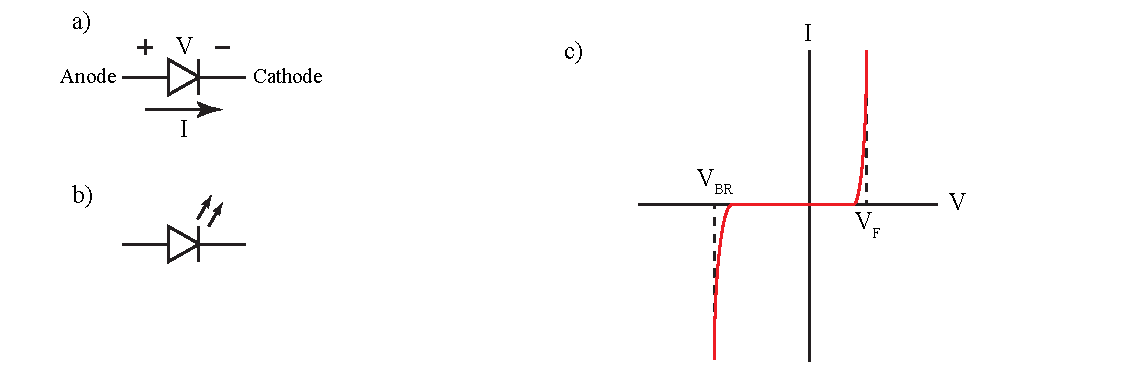
\includegraphics[width=1\textwidth]{Lab6idealDiodes.pdf}
	\caption{Diode schematic symbol with the anode and cathode labeled (a), schematic symbol for an LED (b), and the I-V curve for a diode (c).} \label{fig:idealDiode}
\end{figure}



%%%%%%%%%%%%%%%%%%%%%%%%%%%%%%%%%%%%%%%%%%%%%%%%%%%%%%%%%%%%%%%%%%%%%%%%%%%%%%%%%%%%%%%%%%%%%%%%%%%%%%%
\subsection{Applications}
%%%%%%%%%%%%%%%%%%%%%%%%%%%%%%%%%%%%%%%%%%%%%%%%%%%%%%%%%%%%%%%%%%%%%%%%%%%%%%%%%%%%%%%%%%%%%%%%%%%%%%%

There are a variety of applications for diodes and this lab will focus on only a few, rectifications and clip detection.

%%%%%%%%%%%%%%%%%%%%%%%%%%%%%%%%%%%%%%%%%%%%%%%%%%%%%%%%%%%%%%%%%%%%%%%%%%%%%%%%%%%%%%%%%%%%%%%%%%%%%%%
\subsubsection{Rectifiers}
%%%%%%%%%%%%%%%%%%%%%%%%%%%%%%%%%%%%%%%%%%%%%%%%%%%%%%%%%%%%%%%%%%%%%%%%%%%%%%%%%%%%%%%%%%%%%%%%%%%%%%%

Signal rectification is the process of converting an alternating signal in to its positive or negative components. \hyperref[fig:rect]{Figure \ref*{fig:rect}} is an example of a simple half-wave rectifier. After the input sine wave passes the diodes forward bias voltage, $\approx 0.7$ V, the diode conducts and passes the positive half of the sine wave but doesn't pass the negative half of the sine wave because the diode is reverse bias and does not conduct.

\begin{figure} [h!]
	\centering
		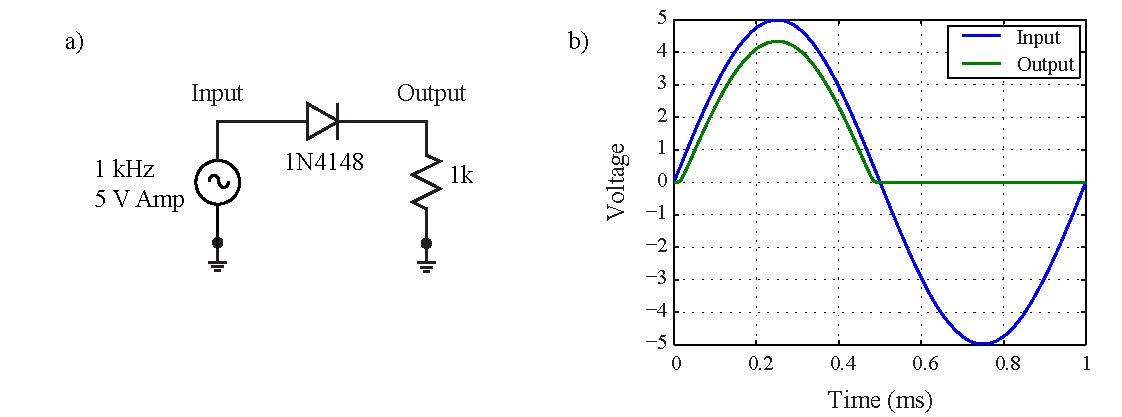
\includegraphics[width=1\textwidth]{Lab6halfrect.pdf}
	\caption{A simple half wave rectifier (a) and the resulting input and output signals (b). } \label{fig:rect}
\end{figure}

Simply adding a capacitor to the half-wave rectifier results in an AC to DC converter, \hyperref[fig:rectWcap]{Figure \ref*{fig:rectWcap}}. The circuit initially behaves as it did previously, once the input sine wave reaches the forward bias voltage, the output follows the input. However, once the sine wave starts to decrease, the output then discharges as a function of an RC time constant, the process then repeats. For higher input frequencies and capacitances, the output cap be approximated as a DC source. 

\begin{figure} [h!]
	\centering
		\includegraphics[width=1\textwidth]{Lab8halfrectWcap.pdf}
	\caption{A simple half wave rectifier but with a capacitor at the output (a) and the resulting input and output signals (b).} \label{fig:rectWcap}
\end{figure}


%%%%%%%%%%%%%%%%%%%%%%%%%%%%%%%%%%%%%%%%%%%%%%%%%%%%%%%%%%%%%%%%%%%%%%%%%%%%%%%%%%%%%%%%%%%%%%%%%%%%%%%
\subsubsection{Clip Detection}
%%%%%%%%%%%%%%%%%%%%%%%%%%%%%%%%%%%%%%%%%%%%%%%%%%%%%%%%%%%%%%%%%%%%%%%%%%%%%%%%%%%%%%%%%%%%%%%%%%%%%%%

There are often cases where the input or output of a system isn't easily accessible for test equipment. A variety of dials, indicators, and display panels are often used to report on the status of a system, examples include current draw, internal voltages, and clip detection. 

Clip detection is the process of determining if a signal is clipping or not. A signal that is clipped, unless desired, can degraded the performance of the system. A clipping detection circuit is able to indicate that the output of the op amp is clipping without viewing the output on an o-scope, but instead through an LED. 

\begin{figure} [h]
	\centering
		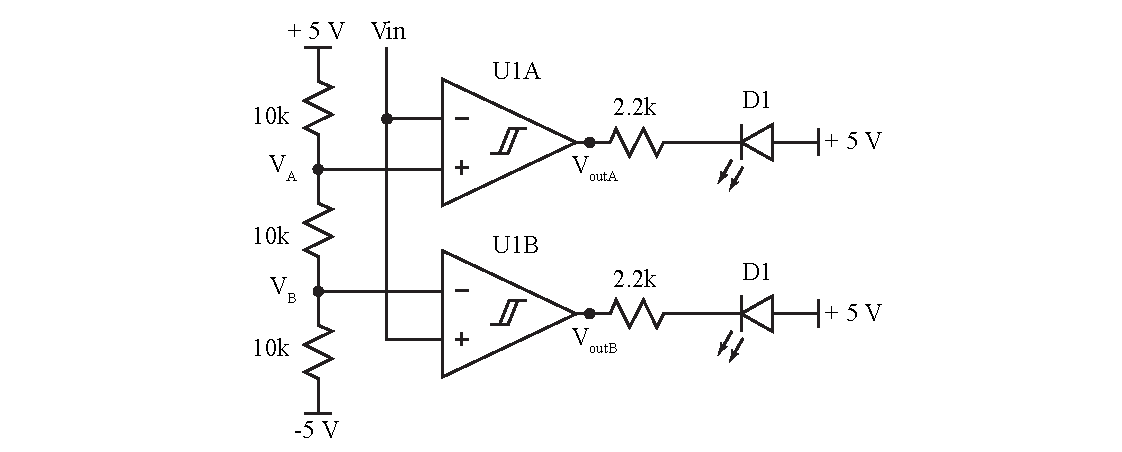
\includegraphics[width=1\textwidth]{Lab6compLED.pdf}
	\caption{A clipping detection circuit. The input is compared to fixed voltages, $V_A$ and $V_B$, by U1A and U1B respectively. If the input voltage is greater, or less, than the reference voltage, the output is pulled low and LED is illuminated.} \label{fig:clipdetect}
\end{figure}

\hyperref[fig:clipdetect]{Figure \ref*{fig:clipdetect}} is an example of a clipping detector. If the input is higher, or lower, than the reference voltage $V_A$, or $V_B$, the LED D1, or D2, illuminates indicated that the input voltage is above, or below, the reference voltage. Note that this circuit does not use op amps, but comparators. Comparators, as the name implies, compares the input at both terminals and produces a digital output, either a 1 (5 V) or 0 (0V), if the positive terminal input is larger than the negative terminal input. 


%%%%%%%%%%%%%%%%%%%%%%%%%%%%%%%%%%%%%%%%%%%%%%%%%%%%%%%%%%%%%%%%%%%%%%%%%%%%%%%%%%%%%%%%%%%%%%%%%%%%%%
\subsection{Potentiometers}
%%%%%%%%%%%%%%%%%%%%%%%%%%%%%%%%%%%%%%%%%%%%%%%%%%%%%%%%%%%%%%%%%%%%%%%%%%%%%%%%%%%%%%%%%%%%%%%%%%%%%%

A potentiometer (or ``pot'') is a three terminal resistor as shown in \hyperref[fig:potcktdia]{Figure \ref*{fig:potcktdia}}. The resistance between terminals 1 and 3 is fixed and is equal to the rated value for the potentiometer. Terminal 2 is connected to a movable contact called the arm or wiper and the resistance between terminals 2 and 1 or between 2 and 3 can be varied by moving the arm. If terminals 1 and 3 are connected across a voltage source, then the voltage between terminals 2 and 1 or between 2 and 3 can be varied by moving the arm. In some cases, terminal 2 is connected to either terminal 1 or 3 so that the resistance from terminals 1 to 3 can be varied. 

\begin{figure}[h] 
	\centering
	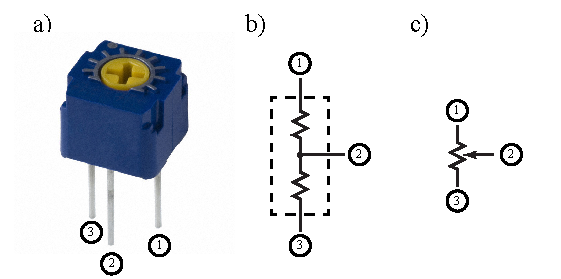
\includegraphics[width=0.5\textwidth]{lab6potdia.pdf}
	\caption{A picture of a practical potentiometer with the appropriate pins labeled (a), an equivalent circuit diagram of a potentiometer with the wiper in a fixed position (b), and the common circuit schematic representation for a potentiometer (c).} \label{fig:potcktdia}
\end{figure}

The potentiometer model in spice is as simple a single resistor, with a resistance equal to the total resistance or less than the total resistance, where the values changes simulation to simulation to the desired resistance. 

%%%%%%%%%%%%%%%%%%%%%%%%%%%%%%%%%%%%%%%%%%%%%%%%%%%%%%%%%%%%%%%%%%%%%%%%%%%%%%%%%%%%%%%%%%%%%%%%%%%%%%%
\section{Big Picture}
%%%%%%%%%%%%%%%%%%%%%%%%%%%%%%%%%%%%%%%%%%%%%%%%%%%%%%%%%%%%%%%%%%%%%%%%%%%%%%%%%%%%%%%%%%%%%%%%%%%%%%%

\begin{figure} [h]
	\centering
		\includegraphics[width=1\textwidth]{Lab8bigpicture.pdf}
	\caption{Big picture with emphasis on the peak detector.} \label{fig:8bp}
\end{figure}

This lab focuses on diode circuits which will help to form the comparator circuits used in the peak detector for the final project. 

%%%%%%%%%%%%%%%%%%%%%%%%%%%%%%%%%%%%%%%%%%%%%%%%%%%%%%%%%%%%%%%%%%%%%%%%%%%%%%%%%%%%%%%%%%%%%%%%%%%%%%%
\section{Pre-Lab Requirements}
%%%%%%%%%%%%%%%%%%%%%%%%%%%%%%%%%%%%%%%%%%%%%%%%%%%%%%%%%%%%%%%%%%%%%%%%%%%%%%%%%%%%%%%%%%%%%%%%%%%%%%%

Complete the following before coming to lab. 

%%%%%%%%%%%%%%%%%%%%%%%%%%%%%%%%%%%%%%%%%%%%%%%%%%%%%%%%%%%%%%%%%%%%%%%%%%%%%%%%%%%%%%%%%%%%%%%%%%%%%%%
\subsection{LTspice Simulations} \label{ssec:6spice}
%%%%%%%%%%%%%%%%%%%%%%%%%%%%%%%%%%%%%%%%%%%%%%%%%%%%%%%%%%%%%%%%%%%%%%%%%%%%%%%%%%%%%%%%%%%%%%%%%%%%%%%

Using LTspice, complete the following.

\begin{enumerate}
	\item Build the circuit in \hyperref[fig:rect]{Figure \ref*{fig:rect} (a)}. Set the input to a 1 kHz, 5 V amplitude sine wave and run a transient simulation with a stop time of 1m (.tran 1m) and plot the input and output.  To use the 1N4148 diode model, right click on the diode after placing it, Pick New Diode, and then choose the 1N4148 model (Mfg. OnSemi). Save an image of the circuit and the plot of the input and output voltage for submission to canvas. \label{itm:8ssec1itm1}
	\item Build the circuit in \hyperref[fig:rectWcap]{Figure \ref*{fig:rectWcap} (a)}. Set the input to a 100 kHz, 5 V amplitude sine wave and run a transient simulation with a stop time of 50u (.tran 50u) and step through possible capacitor values using the following spice directive:
			\begin{verbatim}
			.step param C list 0.001u 0.01u 0.1u 1u
		\end{verbatim}
	 Save an image of the circuit and the plot of the input and output voltage for submission to canvas. \label{itm:8ssec1itm2}
	\item Build the circuit in \hyperref[fig:clipdetect]{Figure \ref*{fig:clipdetect}}. Use the default LED model in LTSpice, and download "slcj016.zip" file from Canvas "Lab Related Files" folder for the LM393 comparator model. Don't use the  "slcj016b.zip" for the comparator model from TI because it's a newer model that doesn't work for input higher than (Vcc-2V). Power the LM393 with +/-5 V. Set the input voltage to a 1 kHz, 5 V amplitude sine wave and run a transient solution with a stop time of 2m (.tran 2m). Plot the input voltage and the current through each diode. Save an image of the circuit and the plot for submission to canvas. \label{itm:8ssec1itm3}
	\item Build the circuit in \hyperref[fig:vga]{Figure \ref*{fig:vga}}. Power the LM393 and TLV272 with  +/-5 V. Set the input voltage to a 1kHz, 0.1 V amplitude sine wave and run a transient solution with a stop time of 2m. Choose the value for R1, 10k pot, so that the diodes conduct current and illuminate. Plot the input voltage, output of the op amp, positive and negative inputs to the comparator, and the current through both LEDs. (6 items total). Save an image of the circuit and the plot for submission to canvas. \label{itm:8ssec1itm4}
\end{enumerate}

\begin{figure}[h] 
	\centering
	\includegraphics[width=1\textwidth]{lab6vga.pdf}
	\caption{A variable gain amplifier, R1 is a potentiometer that can be varied, where the output is checked for clipping.} \label{fig:vga}
\end{figure}


%%%%%%%%%%%%%%%%%%%%%%%%%%%%%%%%%%%%%%%%%%%%%%%%%%%%%%%%%%%%%%%%%%%%%%%%%%%%%%%%%%%%%%%%%%%%%%%%%%%%%%%
\subsection{Breadboard Implementation} \label{ssec:6breadboard}
%%%%%%%%%%%%%%%%%%%%%%%%%%%%%%%%%%%%%%%%%%%%%%%%%%%%%%%%%%%%%%%%%%%%%%%%%%%%%%%%%%%%%%%%%%%%%%%%%%%%%%%

\begin{enumerate}
\item Read the datasheet for the LM393, \url{http://www.ti.com/product/LM393/technicaldocuments}. 
\item Build the circuit in \hyperref[fig:clipdetect]{Figure \ref*{fig:clipdetect}} on a breadboard. It is important to note that the pinout for the comparator chip is the same as the op amp. It works differently, but should be connected the same as the op amp. This means you should still connect pin 8 to +5V and pin 4 to -5V (not GND) just as you have done with the opamp.  Set the input to a 0.5 Hz, 5 V amplitude sine wave. Use the two red LEDS in your lab kit, they're bagged separately. The anode for the LEDs is the longer of the two leads. The diodes will illuminate whenever the input voltage is above or below the reference voltage and should appear to blink in turn. Save the circuit to show your lab instructor at the start of lab. \label{itm:8ssec2itm1}
\end{enumerate}

%%%%%%%%%%%%%%%%%%%%%%%%%%%%%%%%%%%%%%%%%%%%%%%%%%%%%%%%%%%%%%%%%%%%%%%%%%%%%%%%%%%%%%%%%%%%%%%%%%%%%%%
\section{In-Lab Requirements}
%%%%%%%%%%%%%%%%%%%%%%%%%%%%%%%%%%%%%%%%%%%%%%%%%%%%%%%%%%%%%%%%%%%%%%%%%%%%%%%%%%%%%%%%%%%%%%%%%%%%%%%

The following must be completed at the start of lab. 

\begin{enumerate}
	\item \hyperref[ssec:6spice]{Section \ref*{ssec:6spice}}
		\begin{enumerate}
			\item \hyperref[itm:8ssec1itm1]{Item \ref*{itm:8ssec1itm1}}: Half wave rectifier, image of the circuit and the plot of the input and output voltage.
			\item \hyperref[itm:8ssec1itm2]{Item \ref*{itm:8ssec1itm2}}: Half wave rectifier with output smoothing, image of the circuit and the plot of the input and output voltage.
			\item \hyperref[itm:8ssec1itm3]{Item \ref*{itm:8ssec1itm3}}: Clipping circuit, image of the circuit and the plot.
			\item \hyperref[itm:8ssec1itm4]{Item \ref*{itm:8ssec1itm4}}: Variable gain amplifier with clip detector, image of the circuit and the plot.
		\end{enumerate}
	\item \hyperref[ssec:6breadboard]{Section \ref*{ssec:6breadboard}}
		\begin{enumerate}
			\item \hyperref[itm:8ssec1itm5]{Item \ref*{itm:8ssec2itm1}}: Operational clipping circuit. 
		\end{enumerate}
\end{enumerate}

%%%%%%%%%%%%%%%%%%%%%%%%%%%%%%%%%%%%%%%%%%%%%%%%%%%%%%%%%%%%%%%%%%%%%%%%%%%%%%%%%%%%%%%%%%%%%%%%%%%%%%%
\subsection{Breadboard Implementation}
%%%%%%%%%%%%%%%%%%%%%%%%%%%%%%%%%%%%%%%%%%%%%%%%%%%%%%%%%%%%%%%%%%%%%%%%%%%%%%%%%%%%%%%%%%%%%%%%%%%%%%%

\begin{enumerate}
\item Plot the input voltage and the voltage at the output of either comparator, \hyperref[fig:clipdetect]{Figure \ref*{fig:clipdetect}}, on the o-scope and save an image of the display. 
	\item Build the circuit from \hyperref[itm:8ssec1itm1]{Section \ref*{ssec:6spice} - Item \ref*{itm:8ssec1itm1}}. Plot the input and output on the o-scope and save an image of the display.
	\item Build two version of the circuit from \hyperref[itm:8ssec1itm2]{Subsection \ref*{ssec:6spice} - Item \ref*{itm:8ssec1itm2}}, one with where the capacitance is 0.1 uF and the other is 0.01 uF. Plot the outputs of both circuits on the o-scope and save an image of the display. 
	\item Build the circuit from \hyperref[itm:8ssec1itm3]{Subsection \ref*{ssec:6spice} - Item \ref*{itm:8ssec1itm4}}. Set the input to a 0.5 Hz, 0.1 V amplitude sine wave. Vary the potentiometer, increase the gain, so that the LEDs illuminate when the op amp output is greater than the reference voltages. Plot the output of the gain amplifier and the output of either comparator on the o-scope and save an image of the display.
\end{enumerate}


%%%%%%%%%%%%%%%%%%%%%%%%%%%%%%%%%%%%%%%%%%%%%%%%%%%%%%%%%%%%%%%%%%%%%%%%%%%%%%%%%%%%%%%%%%%%%%%%%%%%%%%
\section{Write Up}
%%%%%%%%%%%%%%%%%%%%%%%%%%%%%%%%%%%%%%%%%%%%%%%%%%%%%%%%%%%%%%%%%%%%%%%%%%%%%%%%%%%%%%%%%%%%%%%%%%%%%%%

This write up is different than previous write ups. Instead of comparing ideal and non-ideal values, discuss the operation and limitations of each circuit. For example, the first circuit is limited by forward voltage which limits how much of the signal can be rectified. Backup your discussion with images, all four, from the in-lab portion. Also, include diagrams for each circuit, typically this is not required but for this lab circuit diagrams are required. Do not copy the circuit diagrams from the lab manual, create your own, either digitally or by hand. 





\chapter{Lab 9 - Filters}

%%%%%%%%%%%%%%%%%%%%%%%%%%%%%%%%%%%%%%%%%%%%%%%%%%%%%%%%%%%%%%%%%%%%%%%%%%%%%%%%%%%%%%%%%%%%%%%%%%%%%%%
\section{Objective}
%%%%%%%%%%%%%%%%%%%%%%%%%%%%%%%%%%%%%%%%%%%%%%%%%%%%%%%%%%%%%%%%%%%%%%%%%%%%%%%%%%%%%%%%%%%%%%%%%%%%%%%

The objective of this lab is to introduce the concept of filters and explore their applications through examples of passive and active filters. 

%%%%%%%%%%%%%%%%%%%%%%%%%%%%%%%%%%%%%%%%%%%%%%%%%%%%%%%%%%%%%%%%%%%%%%%%%%%%%%%%%%%%%%%%%%%%%%%%%%%%%%
\section{Materials}
%%%%%%%%%%%%%%%%%%%%%%%%%%%%%%%%%%%%%%%%%%%%%%%%%%%%%%%%%%%%%%%%%%%%%%%%%%%%%%%%%%%%%%%%%%%%%%%%%%%%%%%

\begin{itemize}
	\item Laptop with LTSpice
	\item Analog Discovery
	\item Breadboard
	\item Wiring kit
	\item Lab parts kit
\end{itemize}

%%%%%%%%%%%%%%%%%%%%%%%%%%%%%%%%%%%%%%%%%%%%%%%%%%%%%%%%%%%%%%%%%%%%%%%%%%%%%%%%%%%%%%%%%%%%%%%%%%%%%%%
\section{Introduction}
%%%%%%%%%%%%%%%%%%%%%%%%%%%%%%%%%%%%%%%%%%%%%%%%%%%%%%%%%%%%%%%%%%%%%%%%%%%%%%%%%%%%%%%%%%%%%%%%%%%%%%%

Laboratories so far have focused on the time domain. Given a signal with a specific frequency, there is a resulting output that can be viewed with an appropriate time base on the o-scope. Filters are analyzed primary through the frequency domain, where the output is a function of frequency and not time. 

Filters, as the name implies, filters out certain frequencies from passing to the output. There are several types of filters, such lowpass, highpass, bandpass, notch (bandreject), and allpass. While there are applications for all the filter types, there is only enough time to focus on a few, in this case, lowpass and highpass. Additionally, the math associated with filters can become complicated quickly and so only the results will be represented here. 

\begin{figure}
	\centering
		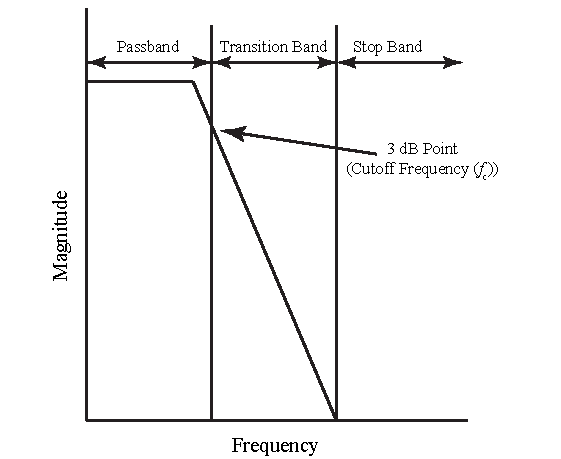
\includegraphics[width=0.5\textwidth]{Lab7FilterResponse.pdf}
	\caption{Example of response for a generic lowpass filter. The filter passes low frequencies frequencies, thus the name, and attenuates higher frequencies. } \label{fig:filterResponse}
\end{figure}

\hyperref[fig:filterResponse]{Figure \ref*{fig:filterResponse}} is an example of a generic lowpass filter response in the frequency domain. The filter, as the name implies, will only pass low frequency signals, higher frequency signals are attenuated through the transition and stop bands. A filter's 3 dB point, cut off frequency, is set by design and is often chosen to obtain a specific attenuation at a certain frequency. Similarly, a high pass filter will behave in the opposite fashion, low frequency signals will be attenuated while high frequency signals will be passed. 

%%%%%%%%%%%%%%%%%%%%%%%%%%%%%%%%%%%%%%%%%%%%%%%%%%%%%%%%%%%%%%%%%%%%%%%%%%%%%%%%%%%%%%%%%%%%%%%%%%%%%%%
\subsection{Passive First Order RC Filters}
%%%%%%%%%%%%%%%%%%%%%%%%%%%%%%%%%%%%%%%%%%%%%%%%%%%%%%%%%%%%%%%%%%%%%%%%%%%%%%%%%%%%%%%%%%%%%%%%%%%%%%%

\hyperref[fig:simpleRC]{Figure \ref*{fig:simpleRC}} shows two simple RC filter configurations and their resulting frequency responses. These filters are considered to be passive, no active elements that require power, and of the first order, there's only one combination of resistors and capacitors. 

\begin{figure}[h]
	\centering
		\includegraphics[width=1\textwidth]{Lab9RCFilters.pdf}
	\caption{An example of a simple RC low pass filter (a) and the resulting frequency response (b). Also, a simple RC highpass filter (c) and the resulting frequency response (d).} \label{fig:simpleRC}
\end{figure}

While the configurations may seem puzzling at first, their results come easily when considering the effects at low and high frequencies. At low frequency, a capacitor acts as an open circuit, $\frac{1}{j\omega C}$ is large when $\omega =2\pi f$ is small, while at high frequencies, it acts as a short circuit, $\frac{1}{j\omega C}$ is small when $\omega$ is large. So, for a lowpass, it makes sense that low frequencies are passed while high frequencies are attenuated. Similarly, for a highpass filter, low frequencies are attenuated while high frequencies are passed. 

There are a variety of equations relating the transfer function of a filter, but instead the focus is on the important parameters. In the case of a simple RC filter, the 3 dB point, or the frequency where the output has dropped to half of the input, is governed by the following equation:

\begin{equation}
f_c = \frac{1}{2 \pi RC}
\end{equation}

\noindent For the examples in \hyperref[fig:simpleRC]{Figure \ref*{fig:simpleRC} (a) and (c)}, the 3 dB point is calculated to be $\frac{1}{2 \pi 10\mathrm{k}\; 0.001\mu} = 15.916\;\mathrm{kHz}$. Which matches the frequency response for both configurations. 

%%%%%%%%%%%%%%%%%%%%%%%%%%%%%%%%%%%%%%%%%%%%%%%%%%%%%%%%%%%%%%%%%%%%%%%%%%%%%%%%%%%%%%%%%%%%%%%%%%%%%%%
\subsection{Active RC Filters}
%%%%%%%%%%%%%%%%%%%%%%%%%%%%%%%%%%%%%%%%%%%%%%%%%%%%%%%%%%%%%%%%%%%%%%%%%%%%%%%%%%%%%%%%%%%%%%%%%%%%%%%

There are a variety of active filter topologies but a simple implementation is to use an appropriately placed capacitor in conjunction with a typical inverting amplifier configuration, \hyperref[fig:9activeRC]{Figure \ref*{fig:9activeRC} (a) and (b)}.

\begin{figure}[h]
	\centering
		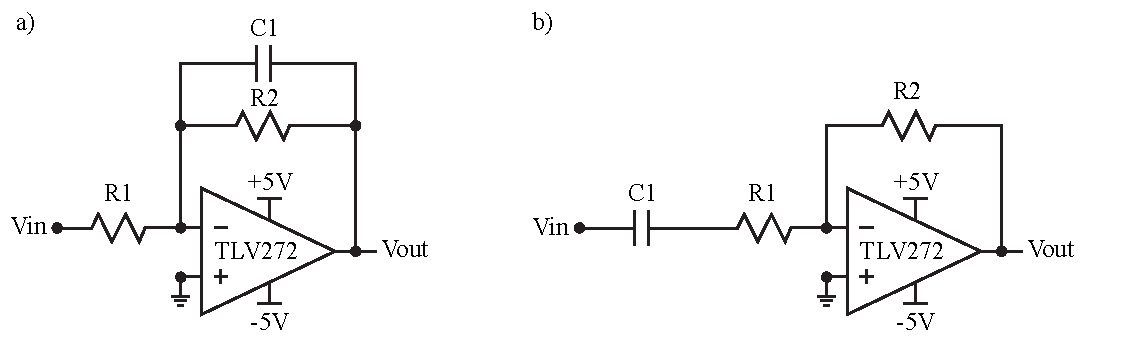
\includegraphics[width=1\textwidth]{Lab9activeRC.pdf}
	\caption{An example of an active RC low pass filter (a) and an active RC high pass filter (b).} \label{fig:9activeRC}
\end{figure}

The design of either the active RC low pass or high pass is also fairly simple for the first order case. A low pass filter has the following equations

\begin{align*}
	\frac{V_{OUT}}{V_{IN}} &= -\frac{R_2}{R_1}\frac{1}{j\omega C_1 R_2 +1} \\
	H_0 &= -\frac{R_2}{R_1} \\
	f_0 &= \frac{1}{2 \pi C_1 R_2} \\
\end{align*}

\noindent where $H_0$ is the passband gain and $f_0$ is the 3dB frequency. Note that unlike the passive RC case, filters using op amps can also have gain. Similarly, the high pass filter has the following equations

\begin{align*}
	\frac{V_{OUT}}{V_{IN}} &= -\frac{R_2}{R_1}\frac{j\omega C_1 R_1}{j\omega C_1 R_1 +1}\\ 
	H_0 &= -\frac{R_2}{R_1}\\
	f_0 &= \frac{1}{2 \pi C_1 R_1}\\
\end{align*}


%%%%%%%%%%%%%%%%%%%%%%%%%%%%%%%%%%%%%%%%%%%%%%%%%%%%%%%%%%%%%%%%%%%%%%%%%%%%%%%%%%%%%%%%%%%%%%%%%%%%%%%%
%\subsection{Active RC Filters - Sallen-Key}
%%%%%%%%%%%%%%%%%%%%%%%%%%%%%%%%%%%%%%%%%%%%%%%%%%%%%%%%%%%%%%%%%%%%%%%%%%%%%%%%%%%%%%%%%%%%%%%%%%%%%%%%
%
%There are a variety of active filter oligopolies but one of the most poplar is the Sallen-Key topology, named after R. P. Sallen and E. L. Key, because the filter depends on the external components and not the op amp. \hyperref[fig:sallenKey]{Figure \ref*{fig:sallenKey}} shows the lowpass and highpass configurations. 
%
%\begin{figure}
	%\centering
		%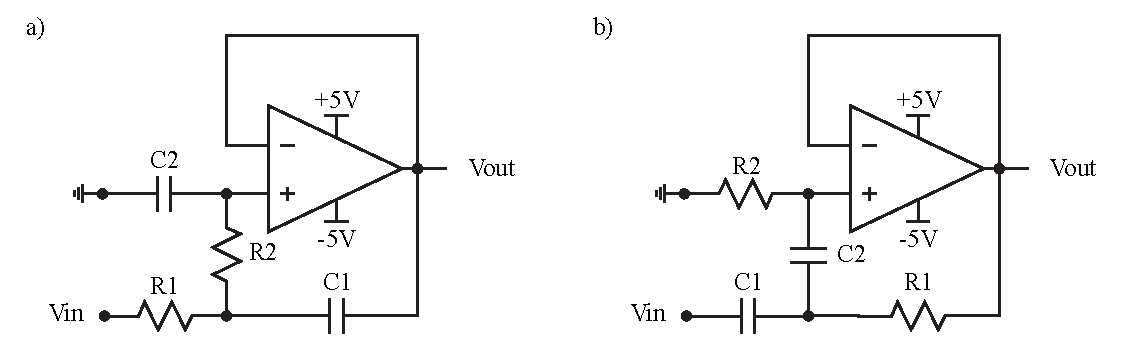
\includegraphics[width=1\textwidth]{lab7sallenkey.pdf}
	%\caption{A Sallen-Key lowpass filter (a) and highpass (b). Note that this is a simplified topology with unity gain.} \label{fig:sallenKey}
%\end{figure}
%
%The design of this filter is more complicated than the simple RC and requires a bit of foresight. For a lowpass, choose C1 and then calculated the other values using the following coefficients and equations
%
%\begin{subequations}
%\	\begin{align}
		%k &= 2\pi f_0 C_1 \\
		%m &= \frac{\alpha^2}{4} \\
		%C_2 &= m C_1 \\
		%R_1 &= \frac{2}{\alpha k} \\
		%R_2 &= \frac{\alpha}{2 m k} 
	%\end{align}
%\end{subequations}
%
%\noindent where $f_0$ is the desired 3 dB point in Hz and $\alpha = 1.4142$ for a second order filter. If the desired $f_0$ is 10 kHz and C1 is chosen to be $0.01\; \mu$F, the remaining values are C2 = $0.005\;\mu$F and R1 = R2 = 2.25 k$\Omega$.
%
%The design equations for a Sallen-Key highpass are similar:
%
%\begin{subequations}
%\	\begin{align}
		%k &= 2\pi f_0 C_1 \\
		%C_2 &= C_1 \\
		%R_1 &= \frac{2\alpha}{4k} \\
		%R_2 &= \frac{4}{2\alpha}\frac{1}{k}
	%\end{align}
%\end{subequations}
%
%\noindent where $f_0$ is the desired 3 dB point in Hz and $\alpha = 1.4142$ for a second order filter. Consider a similar design where $f_0$ is 10 kHz and C1 is chosen to be $0.01\; \mu$F, the remaining values are C2 = $0.01\; \mu$F and R1 = 1.25 k$\Omega$ and R2 = 2.25 k$\Omega$.

%%%%%%%%%%%%%%%%%%%%%%%%%%%%%%%%%%%%%%%%%%%%%%%%%%%%%%%%%%%%%%%%%%%%%%%%%%%%%%%%%%%%%%%%%%%%%%%%%%%%%%%
\section{Big Picture}
%%%%%%%%%%%%%%%%%%%%%%%%%%%%%%%%%%%%%%%%%%%%%%%%%%%%%%%%%%%%%%%%%%%%%%%%%%%%%%%%%%%%%%%%%%%%%%%%%%%%%%%

\begin{figure} [h]
	\centering
		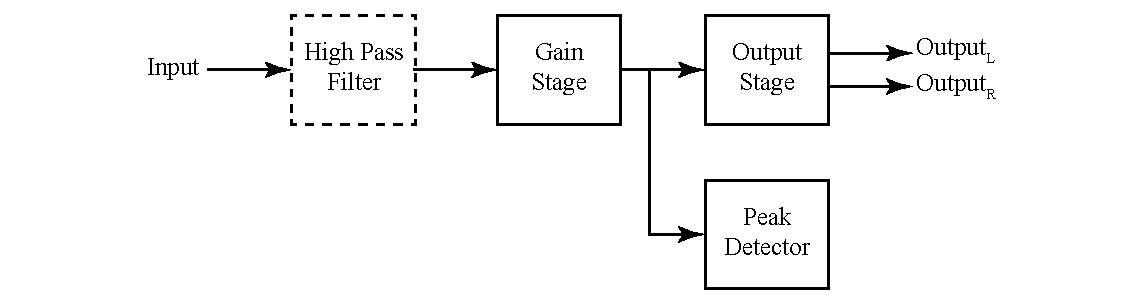
\includegraphics[width=1\textwidth]{Lab9bigpicture.pdf}
	\caption{Big picture with emphasis on the high pass filter.} \label{fig:9bp}
\end{figure}

This lab focuses on filter circuits which will help to create the high pass filter used in the final project used to remove the large DC offset in the source signal. 

%%%%%%%%%%%%%%%%%%%%%%%%%%%%%%%%%%%%%%%%%%%%%%%%%%%%%%%%%%%%%%%%%%%%%%%%%%%%%%%%%%%%%%%%%%%%%%%%%%%%%%%
\section{Pre-Lab Requirements}
%%%%%%%%%%%%%%%%%%%%%%%%%%%%%%%%%%%%%%%%%%%%%%%%%%%%%%%%%%%%%%%%%%%%%%%%%%%%%%%%%%%%%%%%%%%%%%%%%%%%%%%

Complete the following before coming to lab. 

%%%%%%%%%%%%%%%%%%%%%%%%%%%%%%%%%%%%%%%%%%%%%%%%%%%%%%%%%%%%%%%%%%%%%%%%%%%%%%%%%%%%%%%%%%%%%%%%%%%%%%%
\subsection{LTspice Simulations} \label{ssec:9spice}
%%%%%%%%%%%%%%%%%%%%%%%%%%%%%%%%%%%%%%%%%%%%%%%%%%%%%%%%%%%%%%%%%%%%%%%%%%%%%%%%%%%%%%%%%%%%%%%%%%%%%%%

Complete the following using the TLV271 spice model, always power the op amp with +/- 5 V for $V_{dd+}$ and $V_{dd-}$.

\begin{enumerate}
\item Review the LTspice tutorial for AC Analysis, \url{https://www.youtube.com/watch?v=fziUQaVQxA4&t=1s}.
	\item Build a simple lowpass filter, \hyperref[fig:simpleRC]{Figure \ref*{fig:simpleRC} (a)}, but set R = 10 k$\Omega$ and C = $0.001\; \mu$F. Set the voltage source to an AC amplitude of 1 and run an AC analysis with the following settings: Decade, 100, 1, 1Meg. Save an image of the circuit, a plot of the output, and table the 3 dB frequency for submission to Canvas. \label{itm:9ssec1itm1}
	\item Build a simple highpass filter, \hyperref[fig:simpleRC]{Figure \ref*{fig:simpleRC} (c)}, but set R = 15 k$\Omega$ and C = $0.01\; \mu$F. Set the voltage source to an AC amplitude of 1 and run an AC analysis with the following settings: Decade, 100, 1, 1Meg. Save an image of the circuit, a plot of the output, and table the 3 dB frequency for submission to Canvas. \label{itm:9ssec1itm2}
	\item Build an active RC lowpass filter, \hyperref[fig:9activeRC]{Figure \ref*{fig:9activeRC} (a)}. Set $C_1 = 0.1\mu$F and determine the resistor values for a gain of -1 V/V (0 dB) and a $f_0 = 1.59\;\mathrm{kHz}$ using only values in your lab kit. Set the voltage source to an AC amplitude of 1 and run an AC analysis with the following settings: Decade, 100, 1, 1Meg. Save an image of the circuit, a plot of the output, and table the 3 dB frequency for submission to Canvas. \label{itm:9ssec1itm3}
	\item Build an active RC highpass filter, \hyperref[fig:9activeRC]{Figure \ref*{fig:9activeRC} (b)}. Set $C_1 = 0.1\mu$F and determine the resistor values for a gain of -10 V/V (20 dB) and a $f_0 = 482.3\;\mathrm{Hz}$ using only values in your lab kit. Set the voltage source to an AC amplitude of 1 and run an AC analysis with the following settings: Decade, 100, 1, 1Meg. Table the 3 dB frequency. Save an image of the circuit, a plot of the output, and table the 3 dB frequency (3 dB from the passband) for submission to Canvas. \label{itm:9ssec1itm4}
\end{enumerate}

%%%%%%%%%%%%%%%%%%%%%%%%%%%%%%%%%%%%%%%%%%%%%%%%%%%%%%%%%%%%%%%%%%%%%%%%%%%%%%%%%%%%%%%%%%%%%%%%%%%%%%%
\subsection{Breadboard implementation} \label{ssec:9breadboard}
%%%%%%%%%%%%%%%%%%%%%%%%%%%%%%%%%%%%%%%%%%%%%%%%%%%%%%%%%%%%%%%%%%%%%%%%%%%%%%%%%%%%%%%%%%%%%%%%%%%%%%%

\begin{enumerate}
	\item Review the Digilent tutorial for the Network Analyzer tool: \url{https://www.youtube.com/watch?v=31tq_A_2TcY}.
	\item Build the active RC lowpass filter from \hyperref[itm:9ssec1itm3]{Section \ref*{ssec:9spice} - Item \ref*{itm:9ssec1itm3}} on a breadboard. Use a TLV272 op amp and power it with $\pm$ 5 V rails and wire up the Analog Discovery to use the network analyzer tool. \label{itm:9ssec2itm2}
	\item Set the start frequency to 100 Hz, stop frequency to 100 kHz, and the samples to 100. Connect CH1+ and W1 to the input and CH2+ to the output. Uncheck the box next to channel 1 and leave the remaining settings in their default configuration. Click run once to generate the filter's frequency response. Save the circuit to show your lab instructor at the start of lab. \label{itm:9ssec2itm3}
\end{enumerate}


%%%%%%%%%%%%%%%%%%%%%%%%%%%%%%%%%%%%%%%%%%%%%%%%%%%%%%%%%%%%%%%%%%%%%%%%%%%%%%%%%%%%%%%%%%%%%%%%%%%%%%%
\section{In-Lab Requirements}
%%%%%%%%%%%%%%%%%%%%%%%%%%%%%%%%%%%%%%%%%%%%%%%%%%%%%%%%%%%%%%%%%%%%%%%%%%%%%%%%%%%%%%%%%%%%%%%%%%%%%%%

The following must be completed at the start of lab. 

\begin{enumerate}
	\item \hyperref[ssec:9spice]{Section \ref*{ssec:9spice}}
	\begin{enumerate}
		\item Table of 3 dB frequencies (four values).
		\item \hyperref[itm:9ssec1itm1]{Item \ref*{itm:9ssec1itm1}}: Simple RC lowpass filter - image of the circuit and a plot of the output.
		\item \hyperref[itm:9ssec1itm2]{Item \ref*{itm:9ssec1itm2}}: Simple RC highpass filter - image of the circuit and a plot of the output.
		\item \hyperref[itm:9ssec1itm3]{Item \ref*{itm:9ssec1itm3}}: Active RC lowpass filter - image of the circuit and a plot of the output.
		\item \hyperref[itm:9ssec1itm4]{Item \ref*{itm:9ssec1itm4}}: Active RC highpass filter - image of the circuit and a plot of the output.
	\end{enumerate}
	\item \hyperref[ssec:9breadboard]{Section \ref*{ssec:9breadboard}}
	\begin{enumerate}
		\item \hyperref[itm:9ssec2itm3]{Item \ref*{itm:9ssec2itm3}}: Active RC lowpass filter - image of the circuit and a plot of the output.
	\end{enumerate}
\end{enumerate}

%%%%%%%%%%%%%%%%%%%%%%%%%%%%%%%%%%%%%%%%%%%%%%%%%%%%%%%%%%%%%%%%%%%%%%%%%%%%%%%%%%%%%%%%%%%%%%%%%%%%%%%
\subsection{Practical Implementations}
%%%%%%%%%%%%%%%%%%%%%%%%%%%%%%%%%%%%%%%%%%%%%%%%%%%%%%%%%%%%%%%%%%%%%%%%%%%%%%%%%%%%%%%%%%%%%%%%%%%%%%%

For all active circuits, use a TLV272 op amp and power it with $\pm$ 5 V rails.

\begin{enumerate}
	\item Set the number of samples to 1000 and re-run the network analyzer. Save an image of the output, and measure the 3 dB frequency.
	\item Build the circuit from \hyperref[itm:9ssec1itm1]{Section \ref*{ssec:9spice} - Item \ref*{itm:9ssec1itm1}}, run the network analyzer, measure the 3 dB frequency, and save an image of the output.
	\item Build the circuit from \hyperref[itm:9ssec1itm2]{Section \ref*{ssec:9spice} - Item \ref*{itm:9ssec1itm2}}, run the network analyzer, measure the 3 dB frequency, and save an image of the output.
	\item Build the circuit from \hyperref[itm:9ssec1itm4]{Section \ref*{ssec:9spice} - Item \ref*{itm:9ssec1itm4}}, run the network analyzer (set the amplitude to 100 mV from 1 V and the top to 30 dB for this case), measure the 3 dB frequency, and save an image of the output.
\end{enumerate}

%%%%%%%%%%%%%%%%%%%%%%%%%%%%%%%%%%%%%%%%%%%%%%%%%%%%%%%%%%%%%%%%%%%%%%%%%%%%%%%%%%%%%%%%%%%%%%%%%%%%%%%
\section{Write Up}
%%%%%%%%%%%%%%%%%%%%%%%%%%%%%%%%%%%%%%%%%%%%%%%%%%%%%%%%%%%%%%%%%%%%%%%%%%%%%%%%%%%%%%%%%%%%%%%%%%%%%%%

Include the following in the write up.

\begin{itemize}
	\item Table of experimental 3 dB frequencies and their associated percent errors when compared to the pre-lab.
	\item Network analyzer images for each circuit.
\end{itemize}

Discuss the operation of each filter and the difference between the theoretical and experimental 3 dB frequencies and touch on the following topics.

\begin{itemize}
	\item Besides component variation, what other effects continue to shifting the 3 dB frequency from its ideal value?
	\item What are the advantages and disadvantages for each filter type, passive and active?
\end{itemize}


\chapter{Lab 10 - Final Project}

%%%%%%%%%%%%%%%%%%%%%%%%%%%%%%%%%%%%%%%%%%%%%%%%%%%%%%%%%%%%%%%%%%%%%%%%%%%%%%%%%%%%%%%%%%%%%%%%%%%%%%%
\section{Objective}
%%%%%%%%%%%%%%%%%%%%%%%%%%%%%%%%%%%%%%%%%%%%%%%%%%%%%%%%%%%%%%%%%%%%%%%%%%%%%%%%%%%%%%%%%%%%%%%%%%%%%%%

The objective of the final project is to bring together concepts taught in previous labs in to a single circuit. 

%%%%%%%%%%%%%%%%%%%%%%%%%%%%%%%%%%%%%%%%%%%%%%%%%%%%%%%%%%%%%%%%%%%%%%%%%%%%%%%%%%%%%%%%%%%%%%%%%%%%%%%
\section{Materials}
%%%%%%%%%%%%%%%%%%%%%%%%%%%%%%%%%%%%%%%%%%%%%%%%%%%%%%%%%%%%%%%%%%%%%%%%%%%%%%%%%%%%%%%%%%%%%%%%%%%%%%%

\begin{itemize}
	\item Laptop with LTSpice
	\item Analog Discovery
	\item Breadboard
	\item Wiring kit
	\item Lab parts kit with TLV272 and LM393P
	\item Speakers with 3.5mm connector
\end{itemize}

%%%%%%%%%%%%%%%%%%%%%%%%%%%%%%%%%%%%%%%%%%%%%%%%%%%%%%%%%%%%%%%%%%%%%%%%%%%%%%%%%%%%%%%%%%%%%%%%%%%%%%%
\section{Introduction}
%%%%%%%%%%%%%%%%%%%%%%%%%%%%%%%%%%%%%%%%%%%%%%%%%%%%%%%%%%%%%%%%%%%%%%%%%%%%%%%%%%%%%%%%%%%%%%%%%%%%%%%

The nature of the lab will be different to accommodate the final project. With a total score that accounts for 20\% of the entire lab grade, the final project is required to pass the course. There is no quiz for the final project and the breakdown is as follows:

\begin{itemize}
	\item 20\% Pre-lab 
	\item 40\% In-lab Demonstration (This includes building your final circuit on a provided printed circuit board)
	\item 40\% Write up 
	
\end{itemize}

The pre-lab simply requires a working spice schematic with the correct outputs, this is much simpler than it sounds. Source files for the spice simulation are available on Canvas under the Labs folder, Jingle4.wav and Jingle19.wav. The wav files can be imported in to LTspice using the following instructions, \url{http://www.linear.com/solutions/6087}. The final simulation, the simulation that's submitted to Canvas, must use the Jingle19.wav file and a transient simulation that's 19 seconds long (.tran 19). Because of the total time to complete the simulation, several minutes, a shorted file has been provided, Jingle4.wav, which runs for four seconds. 

Failure to complete the pre-lab will result in a zero for 20\% of the final project and being barred from the first lab sessions. A student will not however receive a zero for the entire lap project. 

Lab sessions for the final project will span two weeks and exist purely for the student to demo their working breadboard circuit using the in-lab speakers and connector. Because there isn't enough connectors or speakers for students to take them home, both items must remain in the lab. The deadline to have a circuit checked off is approximately the end of the second lab session. Students are not allowed to demo their circuit during lab sessions that are not their own or during office hours.

The write up for the project is also different, see the template in the files section, and the due time for the final report will be announced in Canvas.


%%%%%%%%%%%%%%%%%%%%%%%%%%%%%%%%%%%%%%%%%%%%%%%%%%%%%%%%%%%%%%%%%%%%%%%%%%%%%%%%%%%%%%%%%%%%%%%%%%%%%%%
\subsection{Audio Amplifier}
%%%%%%%%%%%%%%%%%%%%%%%%%%%%%%%%%%%%%%%%%%%%%%%%%%%%%%%%%%%%%%%%%%%%%%%%%%%%%%%%%%%%%%%%%%%%%%%%%%%%%%%


The final project is a basic audio amplifier with a block diagram shown below in \hyperref[fig:10blockDia]{Figure \ref*{fig:10blockDia}}. A simple jingle with a small amplitude, mV, and a large DC offset, 0.5 V, will serve as the input. The system functions as follows.

\begin{figure}[h]
	\centering
		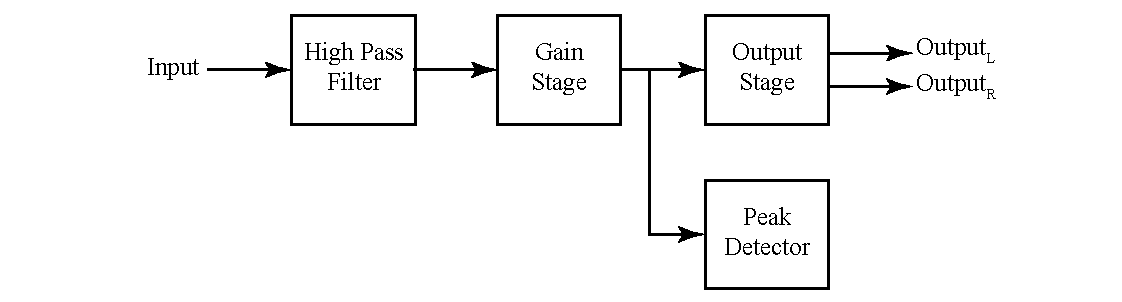
\includegraphics[width=1\textwidth]{Lab10blockdia.pdf}
	\caption{Audio amplifier block diagram. } \label{fig:10blockDia}
\end{figure}

\begin{itemize}
	\item The high pass filter removes the DC offset from the jingle, effectively AC coupling the signal in to the system.
	\item A gain stage is used to amplify the jingle to a range of volts from mV so that it can be heard from the speakers.
	\item An output stage must buffer the output to the speakers, the outputs do not need to be offset in phase.
	\item A peak detector is also required in order to indicate when the output is in the right range, defined by two thresholds. When the output passes the first threshold (LED 1 turns on), the output is operating in the normal linear range with an output on the order of Volts, and the second threshold (LED 2 turns on), where the output is about to start clipping. See the different LED states in \hyperref[tbl:10peakStates]{Table \ref*{tbl:10peakStates}}. Note that this is a slight variation on the circuit used in the diode lab. 
\end{itemize}


\begin{table}
	\centering
\begin{tabular}{| l | l | l |}
	\hline
	\textbf{State} & \textbf{LED 1} & \textbf{LED 2} \\ \hline
	Input < Threshold 1 and 2 & Off & Off \\ \hline
	Threshold 1 < Input < Threshold 2 & On & Off \\ \hline
	Threshold 1 and 2 < Input & On & On \\ \hline
\end{tabular}
	\caption{Different states for the peak detector}
	\label{tbl:10peakStates}
\end{table}

%For the purposes of this class, AM modulation is simple the multiplication of two signals, a high frequency carrier, and a low frequency signal that contains the desired information. The nature of AM modulation results in the low frequency signal forming the envelope of the combined multiplication of the two signals which can be easily extracted using a simple half wave rectifier. 
%
%Unlike a typical AM radio receiver, the input for this circuit will be fixed to the following Wavegen settings, choose \textbf{Modulation} in place of \textbf{Simple} from the pulldown:
%
%\begin{table}[h]
%\begin{center}
%\begin{tabular}{|l|l|l|}
	%\hline
	 %& \textbf{Carrier} & \textbf{Source (AM)} \\ \hline
	%\textbf{Type} & Sine & Sine \\ \hline
	%\textbf{Frequency} & 1.5 MHz & 5 kHz \\ \hline
	%\textbf{Amplitude} / Index: & 1 V & 5\% \\ \hline
	%\textbf{Offset} & 0 V & 0\% \\ \hline
	%\textbf{Symmetry} & 50\% & 50\% \\ \hline
	%\textbf{Phase}: & 0$\deg$ & 0$\deg$ \\ \hline
%\end{tabular}
%\end{center}
%\caption{Wavegen AM modulation settings.}
%\label{tbl:AMwavegen}
%\end{table}
%
%Most of the components have been discussed in previous labs, save for the output stage, and it is up to the student to implement each stage. Beware that there are limited components in your kit, choose your values wisely. A quad op amp chip will also be provided, claim it at office hours or during your lab session.

%%%%%%%%%%%%%%%%%%%%%%%%%%%%%%%%%%%%%%%%%%%%%%%%%%%%%%%%%%%%%%%%%%%%%%%%%%%%%%%%%%%%%%%%%%%%%%%%%%%%%%%
\subsection{Recommendations}
%%%%%%%%%%%%%%%%%%%%%%%%%%%%%%%%%%%%%%%%%%%%%%%%%%%%%%%%%%%%%%%%%%%%%%%%%%%%%%%%%%%%%%%%%%%%%%%%%%%%%%%

\noindent A few words on some of the individual sections. 

\begin{itemize}
	\item As always, you're limited to the components in your lab kit, not the Digilent student kit, choose your values wisely.
	\item Choose the 3dB frequency of the high pass filter carefully. The audio band is 20 Hz to 20 kHz and a 3 dB frequency in the kHz will attenuate (weaken/shrink) important parts of the jingle. Good rule of thumb is if you are over 1 KHz then you are too high. However don't choose it too low, aim for higher than 50 Hz.
	\item The required gain is high, and amplification should occur in two stages. One stage will have a fixed gain. This will be your active high pass filter, both accomplishing the needed filtering and providing gain. The next stage will be another amplifer with variable gain (using a potentiometer as the input resistor). This will allow for a variable voltage on the output signal.
	\item The output stage should be trivial.
	\item Choose the voltage thresholds for the peak detector so that at a reasonable gain, one LED is always on and the other only turns on when the output starts, or is about to start, to clip or distort. 
	\item Use of the active high pass filter for your first stage eliminates the loading effect.
	\item The circuit should pass a demo using sine wave (10mV amplitude, 1KHz, 0,5V DC offset) as input and the peak detection circuit's Threshold 1 and Threshold 2 voltages should be 1V and 4V.  Both LED should be off when the input is <1V, one LED on when the input is between 1V and 4V for OPAMP's linear range operation, then both LEDs should be on when the input is >4V to indicate OPAMP's output is getting into saturation range. The comparator's input configuration is different than Lab 8's, don't copy it directly.
	\item Output stage should have two buffers (for channels L and R).
	\item After you finish the demo and verification of your final project circuits, you need to continue to perform more measurement using scope, spectrum analyzer and network analyzer functions. Follow the file "Final Project Write Up Template" to complete your final report. 
	\item Due time for the final report will be announced in Canvas.  

\end{itemize}

\noindent And some more general advice.

\begin{itemize}
	\item Build everything in LTspice before doing any work on a breadboard. 
	\item The spice simulation of the 19 second jingle file will take a long time, several minutes. The 4 second jingle will also take a few minutes. Start instead with a 10 mV amplitude 1k Hz sine wave with a 0.5 V DC offset and a transient simulation of 1m (.tran 1m). Once you have that working, start using the jingle files. 
	\item Use virtual net nodes instead of making various +5 V and -5 V supplies. 
	\item All of the active components are powered by +5 V and -5 V supplies.
	\item When it's time to build the circuit on a breadboard, build the circuit in a linear fashion. The input should start at one end with the output at the other, don't make it a maze.
	\item Use color coded wires to make debugging easier and avoid creating extra nodes whenever possible. The more nodes in the circuit, the less likely it's going to work.
	\item Build stages one at a time to confirm that they're working as opposed to building everything at once and then trying to debug everything at once. 
	\item Complete the project in the first week, there's a test the second week and it's better to simply get the project out of the way. During the second week you will also need to make time to solder the parts from the project on to a provided PCB for the final demo.
	\item Once you've demoed your circuit, don't take it apart, you'll still need it for items in the write up. It is recommended to complete all measurements required by the write up before soldering to the PCB.
\end{itemize}

%%%%%%%%%%%%%%%%%%%%%%%%%%%%%%%%%%%%%%%%%%%%%%%%%%%%%%%%%%%%%%%%%%%%%%%%%%%%%%%%%%%%%%%%%%%%%%%%%%%%%%%
\section{Pre-Lab Requirements}
%%%%%%%%%%%%%%%%%%%%%%%%%%%%%%%%%%%%%%%%%%%%%%%%%%%%%%%%%%%%%%%%%%%%%%%%%%%%%%%%%%%%%%%%%%%%%%%%%%%%%%%

This following must be completed and submitted to Canvas by the start of lab.

\begin{enumerate}
	\item Image of the spice schematic and a plot of the input and all subsequent outputs (outputs of each individual stage) for a transient simulation for Jingle19 submitted to Canvas. Include the plot of the output and a circuit schematic, nothing else. The schematic and plot should be appropriately labeled. Images that are unclear or vague will receive little to no points. Your plot must include the following in \textbf{different plot planes}: input voltage, output of the high pass filter, output of the variable gain amplifier, output of the buffer stage (at least one), and the current of both LEDs. The gain doesn't need to be high enough to induce clipping in order to show that both LEDs turn on but the first LED should turn on. 
\end{enumerate}

%%%%%%%%%%%%%%%%%%%%%%%%%%%%%%%%%%%%%%%%%%%%%%%%%%%%%%%%%%%%%%%%%%%%%%%%%%%%%%%%%%%%%%%%%%%%%%%%%%%%%%%
\section{In-Lab Requirements}
%%%%%%%%%%%%%%%%%%%%%%%%%%%%%%%%%%%%%%%%%%%%%%%%%%%%%%%%%%%%%%%%%%%%%%%%%%%%%%%%%%%%%%%%%%%%%%%%%%%%%%%

Unlike previous labs, the final project lab spans two weeks (two lab sessions). The final project in-lab portion is only complete once a student has demoed a working circuit. There are two steps to demonstration that a circuit is working:

\begin{enumerate}
	\item Using an input of a 10 mV amplitude sine wave with a 0.5 V DC offset, demonstrate that that the output can be varied and the peak detectors functions properly.
	\item Using the 19 second jingle file as an input, demonstrate that the output can be heard on both speakers and the peak detector functions properly. 
\end{enumerate}

A student can demonstrate their working circuit during either of the two lab sessions, but only in their lab session, not during another lab session or office hours. There are a limited number of connectors and speakers, they will only be handed out to a student once they have demonstrated the first step of the required demonstration.

%%%%%%%%%%%%%%%%%%%%%%%%%%%%%%%%%%%%%%%%%%%%%%%%%%%%%%%%%%%%%%%%%%%%%%%%%%%%%%%%%%%%%%%%%%%%%%%%%%%%%%%
\subsection{Wavegen Settings and Speakers}
%%%%%%%%%%%%%%%%%%%%%%%%%%%%%%%%%%%%%%%%%%%%%%%%%%%%%%%%%%%%%%%%%%%%%%%%%%%%%%%%%%%%%%%%%%%%%%%%%%%%%%%

In order to play the sound file, Jingle19.wav, it must be imported in to the Wavegen's player. Instead of simple, choose play from the pulldown. Click import and then select the Jingle19.wav file. You'll be given a list of options and a plot of the signal, leave the settings to their default and select ok. Hit run to start the jingle playing. 

The 3.5mm connector has three right angle pins soldered to it which allow it to be used with a breadboard. The center pin is ground and the other two pins connect to a speaker. Because the outputs are simply buffered, there's no need for a distinction between left and right. 


%%%%%%%%%%%%%%%%%%%%%%%%%%%%%%%%%%%%%%%%%%%%%%%%%%%%%%%%%%%%%%%%%%%%%%%%%%%%%%%%%%%%%%%%%%%%%%%%%%%%%%%%
%\subsection{Demonstration}
%%%%%%%%%%%%%%%%%%%%%%%%%%%%%%%%%%%%%%%%%%%%%%%%%%%%%%%%%%%%%%%%%%%%%%%%%%%%%%%%%%%%%%%%%%%%%%%%%%%%%%%%
%
%The lab demo consists of the following. Under all conditions, the speaker gain (the volume knob) should be kept to a minimum.
%
%\begin{enumerate}
	%\item Operating of the circuit under normal conditions with the speakers connected. The jingle should be audible on both speakers and the normal LED, case one, should be illuminated. 
	%\item From the previous configuration, the gain is changed in order to induce clipping, which is audible, and should illuminate the other LED, case two. .
%\end{enumerate}

%%%%%%%%%%%%%%%%%%%%%%%%%%%%%%%%%%%%%%%%%%%%%%%%%%%%%%%%%%%%%%%%%%%%%%%%%%%%%%%%%%%%%%%%%%%%%%%%%%%%%%%
\section{Write Up}
%%%%%%%%%%%%%%%%%%%%%%%%%%%%%%%%%%%%%%%%%%%%%%%%%%%%%%%%%%%%%%%%%%%%%%%%%%%%%%%%%%%%%%%%%%%%%%%%%%%%%%%

The write up is also different for the lab project, it takes the form of a formal report. See the template for details. The write up due time will be posted to Canvas, and is typically due around the end of the semester. 












%%%%%%%%%%%%%%%%%%%%%%%%%%%%%%%%%%%%%%%%%%%%%%%%%%%%%%%%%%%%%
%% APPENDICES
%%%%%%%%%%%%%%%%%%%%%%%%%%%%%%%%%%%%%%%%%%%%%%%%%%%%%%%%%%%%%

%% ==> Write your text here or include other files.

%\input{FileName} %You need a file 'FileName.tex' for this.


\end{document}

